\documentclass[onecolumn,10pt]{IEEEtran}
\let\labelindent\relax
\usepackage{enumitem}
%\usepackage{etex}
\newcommand\hmmax{0}
\newcommand\bmmax{0}
\usepackage{amssymb,amsfonts,amsmath,amsthm}
\usepackage{graphicx}
\usepackage[usenames,x11names, dvipsnames, svgnames]{xcolor}
\usepackage{amsmath,amssymb}
\usepackage{dsfont}
\usepackage{amsfonts}
\usepackage{mathrsfs}
\usepackage{hyperref}
\usepackage{makecell}
%\usepackage{bm}
\hypersetup{
  colorlinks=true,
  linkcolor=black,
  citecolor=black,
  filecolor=black,
  urlcolor=DodgerBlue4,
  breaklinks=false,
  % linkbordercolor=red,% hyperlink borders will be red
  % pdfborderstyle={/S/U/W 1}% border style will be underline of width 1pt
}
\usepackage{array}
\usepackage{xr}
\usepackage{verbatim}
\usepackage{multirow}
\usepackage{longtable}
\usepackage{siunitx}
\usepackage{booktabs}
\usepackage{tabularx}
\usepackage{ragged2e}
\usepackage{bm}
\usepackage[size=normal]{subcaption}
\usepackage{pdflscape}
\addtolength{\textwidth}{-.1in}    
\addtolength{\hoffset}{.05in}    
\addtolength{\textheight}{.1in}    
\addtolength{\footskip}{0in}    
\usepackage{rotating}
\usepackage{fancyhdr}
\usepackage{mathtools}
\usepackage{datetime}
\usepackage{comment}
%% ## Equation Space Control---------------------------
\def\EQSP{3pt}
\newcommand{\mltlne}[2][\EQSP]{\begingroup\setlength\abovedisplayskip{#1}\setlength\belowdisplayskip{#1}\begin{equation}\begin{multlined} #2 \end{multlined}\end{equation}\endgroup\noindent}
\newcommand{\cgather}[2][\EQSP]{\begingroup\setlength\abovedisplayskip{#1}\setlength\belowdisplayskip{#1}\begin{gather} #2 \end{gather}\endgroup\noindent}
\newcommand{\cgathers}[2][\EQSP]{\begingroup\setlength\abovedisplayskip{#1}\setlength\belowdisplayskip{#1}\begin{gather*} #2 \end{gather*}\endgroup\noindent}
\newcommand{\calign}[2][\EQSP]{\begingroup\setlength\abovedisplayskip{#1}\setlength\belowdisplayskip{#1}\begin{align} #2 \end{align}\endgroup\noindent}
\newcommand{\caligns}[2][\EQSP]{\begingroup\setlength\abovedisplayskip{#1}\setlength\belowdisplayskip{#1}\begin{align*} #2 \end{align*}\endgroup\noindent}
\newcommand{\mnp}[2]{\begin{minipage}{#1}#2\end{minipage}} 
%% COLOR DEFS------------------------------------------
\newtheorem{thm}{Theorem}
\newtheorem{cor}{Corollary}
\newtheorem{lem}{Lemma}
\newtheorem{prop}{Proposition}
\newtheorem{defn}{Definition}
\newtheorem{exmpl}{Example}
\newtheorem{rem}{Remark}
\newtheorem{notn}{Notation}
%% ------------ -----------------
% color commands------------------------
\newcommand{\etal}{\textit{et} \mspace{3mu} \textit{al.}}
% \renewcommand{\algorithmiccomment}[1]{$/** $ #1 $ **/$}
\newcommand{\vect}[1]{\textbf{\textit{#1}}}
\newcommand{\figfont}{\fontsize{8}{8}\selectfont\strut}
\newcommand{\hlt}{ \bf \sffamily \itshape\color[rgb]{.1,.2,.45}}
\newcommand{\pitilde}{\widetilde{\pi}}
\newcommand{\Pitilde}{\widetilde{\Pi}}
\newcommand{\bvec}{\vartheta}
\newcommand{\algo}{\textrm{\bf\texttt{GenESeSS}}\xspace}
\newcommand{\xalgo}{\textrm{\bf\texttt{xGenESeSS}}\xspace}
\newcommand{\FNTST}{\bf }
\newcommand{\FNTED}{\color{darkgray} \scriptsize $\phantom{.}$}
\renewcommand{\baselinestretch}{.95}
\newcommand{\sync}{\otimes}
\newcommand{\psync}{\hspace{3pt}\overrightarrow{\hspace{-3pt}\sync}}
\newcommand{\base}[1]{\llbracket #1 \rrbracket}
\newcommand{\nst}{\textrm{\sffamily\textsc{Numstates}}}
\newcommand{\HA}{\boldsymbol{\mathds{H}}}
\newcommand{\eqp}{ \vartheta }
\newcommand{\entropy}[1]{\boldsymbol{h}\left ( #1 \right )}
\newcommand{\norm}[1]{\left\lVert #1 \right\rVert}%
\newcommand{\abs}[1]{\left\lvert #1 \right\rvert}%
\newcommand{\absB}[1]{\big\lvert #1 \big\rvert}%
% #############################################################
% #############################################################    
\DeclareMathOperator*{\argmax}{argmax}
\DeclareMathOperator*{\argmin}{arg\,min}
\DeclareMathOperator*{\expect}{\mathbf{E}}
\DeclareMathOperator*{\var}{\mathbf{Var}}
\newcommand{\ND}{ \mathcal{N}  }
\usepackage[linesnumbered,ruled,vlined,noend]{algorithm2e}
\newcommand{\captionN}[1]{\caption{\color{darkgray} \sffamily \fontsize{9}{10}\selectfont #1  }}
\newcommand{\btl}{\ \textbf{\small\sffamily bits/letter}}
\newcolumntype{L}[1]{>{\rule{0pt}{2ex}\raggedright\let\newline\\\arraybackslash\hspace{0pt}}m{#1}}
\newcolumntype{C}[1]{>{\rule{0pt}{2ex}\centering\let\newline\\\arraybackslash\hspace{0pt}}m{#1}}
\newcolumntype{R}[1]{>{\rule{0pt}{2ex}\raggedleft\let\newline\\\arraybackslash\hspace{0pt}}m{#1}}
\newcommand{\set}[1]{\left\{ #1 \right\}}
\newcommand{\paren}[1]{\left( #1 \right)}
\newcommand{\bracket}[1]{\left[ #1 \right]}
% \newcommand{\norm}[1]{\left\Vert #1 \right\Vert}
\newcommand{\nrm}[1]{\left\llbracket{#1}\right\rrbracket}
\newcommand{\parenBar}[2]{\paren{#1\,{\left\Vert\,#2\right.}}}
\newcommand{\parenBarl}[2]{\paren{\left.#1\,\right\Vert\,#2}}
\newcommand{\ie}{$i.e.$\xspace}
\newcommand{\addcitation}{\textcolor{black!50!red}{\textbf{ADD CITATION}}}
\newcommand{\subtochange}[1]{{\color{black!50!green}{#1}}}
\newcommand{\tobecompleted}{{\color{black!50!red}TO BE COMPLETED.}}
\newcommand{\pIn}{\mathscr{P}_{\textrm{in}}}
\newcommand{\pOut}{\mathscr{P}_{\textrm{out}}}
\newcommand{\aIn}[1][\Sigma]{#1_{\textrm{in}}}
\newcommand{\aOut}[1][\Sigma]{#1_{\textrm{out}}}
\newcommand{\xin}[1]{#1_{\textrm{in}}}
\newcommand{\xout}[1]{#1_{\textrm{out}}}
\newcommand{\R}{\mathbb{R}} % Set of real numbers
\newcommand{\F}[1][]{\mathcal{F}_{#1}}
\newcommand{\SR}{\mathcal{S}} % Semiring of sets
\newcommand{\RR}{\mathcal{R}} % Ring of sets
\newcommand{\N}{\mathbb{N}} % Set of natural numbers (0 included)
\newcommand{\Pp}[1][n]{\mathscr{P}^+_{#1}}
\renewcommand{\entropy}[1]{\boldsymbol{h}\left ( #1 \right )}

\def\TPR{\textrm{TPR}\xspace}
\def\TNR{\textrm{TNR}\xspace}
\def\FPR{\textrm{FPR}\xspace}
\def\PPV{\textrm{PPV}\xspace}

\usepackage{textcomp}
\usepackage{colortbl}
\usepackage{array}
\usepackage{courier} 
\usepackage{wrapfig}
\usepackage{pifont}
\usepackage{setspace}
\usepackage{xstring}
\usepackage{xspace}
\usepackage{flushend}
\newcommand{\qn}[1][i]{\Phi_{#1}}
\newcommand{\D}[1][i]{\mathscr{D}\left ( {\Sigma_#1} \right ) }
\newcommand{\Dx}{\mathscr{D}}
\def\J{\mathds{J}}
\def\M{\omega}
\def\N{\mathds{N}}
\newcommand{\cp}[1][P]{\langle #1 \rangle}
\newcommand{\mem}[1]{\M_{#1}}



\usepackage{float}


\def\TITLE{A Digital Twin of the Infant Microbiome to  Predict Neurodevelopmental Deficits}

%\def\TITLE{A Digital Twin of the Infant Microbiome to  Predict Head Circumference Growth}
\title{\TITLE}

\def\x{\bm{\mathrm{x}}} 
\def\y{\bm{\mathrm{y}}}



\author{\sffamily  \fontsize{10}{12}\selectfont Nicholas Sizemore$^{1}$, Kaitlyn Oliphant$^{2}$, Ruolin Zheng$^{1}$, Camilia R. Martin$^{6}$, Erika C. Claud$^{2,3}$ and Ishanu Chattopadhyay$^{1,4,5,7\bigstar}$\\ 
\vspace{10pt}

\sffamily  \fontsize{10}{12}\selectfont
$^{1}$Department of Medicine, University of Chicago, Chicago, IL 60637, USA\\ 
$^{2}$Department of Pediatrics, University of Chicago, Chicago, IL 60637, USA\\
$^{3}$Director, Neonatology Research, University of Chicago, Chicago, IL 60637, USA\\
$^{4}$Committee on Quantitative Methods in Social, Behavioral, and Health Sciences, University of Chicago, Chicago, IL 60637, USA\\
$^{5}$Committee on Genetics, Genomics \& Systems Biology, University of Chicago, Chicago, IL 60637, USA\\
$^{6}$Division of Neonatology, Weill Cornell Medicine, New York, NY 10021, USA\\
$^{7}$Center for Health Statistics, University of Chicago, Chicago, IL 60637, USA
\vskip 1em
$^\bigstar$To whom correspondence should be addressed: e-mail: \href{mailto:ishanu@uchicago.edu}{\texttt{ishanu@uchicago.edu}}.}
\title{\TITLE}


\def\TEXTCOL{gray}



\def\J{\mathds{J}}
\def\M{\omega}
%\newcommand{\mem}[1]{\M_{#1}}
\def\cognet{CogNet\xspace}
\def\qnet{Q-net\xspace}
\def\qdist{q-distance\xspace}
\def\qbiome{Qbiome\xspace}
\def\qsamp{q-sampling\xspace}

\def\x{\bm{\mathrm{x}}}
\def\y{\bm{\mathrm{y}}}
\def\erisk{$M_\delta$\xspace}
\def\RHO{A_\delta}
\def\bact{Bacteroidia\xspace}
\def\actn{Actinobacteria\xspace}
\def\gamm{Gammaproteobacteria\xspace}
\def\ubac{unclassified Bacteria\xspace}
\def\bacl{Bacilli\xspace}
\def\clsd{Clostridia\xspace}
\def\corb{Coriobacteriia\xspace}
\def\verru{Verrucomicrobia\xspace}

\cfoot{\scriptsize\thepage}
\lfoot{} 
\rfoot{} 
\def\EXTENDEDDATA{Supplementary\xspace}
\def\Methods{Materials and Methods}
\def\SPREFIX{S-}
\def\SPREFIX{}
\def\SUPPLEMENTARY{Supplementary\xspace}

\externaldocument{SI}


\begin{document} 
\maketitle 

\subsection*{One Sentence Summary}
Novel generative AI discovers cross-talk among gut-bacteria in infants that might help reduce neurodevelopmental risk.

\subsection*{Abstract}
Despite the recognized gut-brain-axis link~\cite{carlson2018infant}, natural variations in microbial profiles between patients hinder definition of normal abundance ranges~\cite{lozupone2012diversity}, confounding the impact of dysbiosis on infant neurodevelopment. We infer a digital twin of the infant microbiome, 
forecasting ecosystem trajectories from a few initial observations. Using 16S rRNA profiles from 88 preterm infants (398 fecal samples and 32,942 abundance estimates for 91 microbial classes), the model (\qnet) predicts abundance dynamics with $R^2=0.69$.  Contrasting the fit to \qnet{s} of typical versus suboptimal development we can reliably estimate individual deficit risk (\erisk), and identify infants achieving poor future head-circumference growth with  $\approx 76\%$ AUC, $95\%\pm 1.8\% $ PPV at $98\%$ specificity at 30 weeks postmenstrual age. We find that early transplantation might mitigate risk for $\approx 45.2\%$ of the cohort, with potentially negative effects from incorrect supplementation. The \qnet represents a generative AI modeling a dynamic ecosystem, with broad potential applications.


% Dysbiosis in the infant microbiome is linked to impaired cognitive development~\cite{carlson2018infant}. Yet, patient-specific microbiome variations hinder the definition of normal ranges~\cite{lozupone2012diversity}, making the microbial impact on neurodevelopment unclear. This study introduces a digital twin of the infant microbiome, forecasting ecosystem trajectories from initial observations. Using 16S rRNA profiles from 88 preterm infants (398 fecal samples and 32,942 abundance estimates for 91 microbial classes), the model (\qnet) predicts abundance dynamics with $R^2=0.69$. It contrasts digital twins of typically and suboptimally developing infants to estimate individual risk (\erisk) of deviant microbiome growth. These deviations correlate with markers of developmental delays detected in the first 2-4 weeks, categorizing infants by head circumference growth with $\approx 76\%$ AUC, $95\%\pm 1.8\% $ PPV at $98\%$ specificity at 30 weeks postmenstrual age. Furthermore,  early microbial interventions is suggested as possibly mitigating developmental risks for about $45.2\%$ of the cohort, with potentially negative effects from incorrect supplantation profile. Broadly, this work reports  a novel generative AI  modelling a  dynamic microbial ecosystem.

\section*{Introduction}

\IEEEPARstart{T}{he} human microbiome, a complex community hosting trillions of microorganisms such as bacteria, archaea, viruses, and various microbial eukaryotes, plays a crucial role in maintaining general health and homeostasis~\cite{cryan2012mind,pmid26947798}. Increasing evidence suggests that microbial dysbiosis contributes to the development and progression of numerous diseases~\cite{pmid25928420}, ranging from facilitating essential digestive processes~\cite{pmid30680646} to regulating the central nervous system through the microbiota-gut-brain axis~\cite{burokas2015microbiota,lu2018microbiota} (\EXTENDEDDATA Table~\ref{mbiomedisorder}). Despite the wealth of detailed -omics profiles available on various microbiome taxa, our comprehension of the early-life ecosystem development remains limited. While the microbiome's role in brain development~\cite{lu2018microbiota} and the significance of microbial dysbiosis in neuroinflammation and neurodevelopmental disorders have been observed (including in preterm births~\cite{lu2019connection,kang2013,hsiao2013}), the specific mechanistic pathways operating along the gut-brain axis are yet to be fully understood~\cite{oliphant2021bacteroidota}.

Building upon the limited understanding of the early-life microbiome development, researchers have been exploring predictive models that can help in diagnosing and understanding the implications of dysbiosis on various health outcomes in pediatric populations. Predictive models for serious pediatric intestinal diseases, such as necrotizing enterocolitis, have been studied by analyzing the infant microbiome through standard deep learning architectures~\cite{hooven2020multiple,olm2019necrotizing}. Other research has investigated the predictive diagnosis of early childhood cognitive deficits based on observed dysbiosis, typically by comparing the microbiomes of children with and without a target disorder~\cite{laue2020prospective}. However, focusing on subjects already diagnosed with cognitive deficits provides limited insights into potential early clinical interventions. Data-driven identification of the microbial ecosystem's organizational rules presents a formidable challenge~\cite{matchado2021network}; the immense complexity of potential interactions within the microbial ecosystem makes it impractical to discover its organizational rules through experimentation alone, although some targeted experiments for determining causal relationships do exist~\cite{fischbach2018microbiome}. Moreover, the relatively high cost and time-consuming nature of microbiome profile collection result in limited dataset sizes, further complicating automated inference.  Current analyses often concentrate on inferring coarse correlative associations~\cite{faust2016conet,deng2012molecular,friedman2012inferring}, with limited ability to discern subtle predictive patterns and non-linear relationships~\cite{fang2015cclasso,ban2015investigating}. 

The rapid maturation of the infant microbiome, which occurs over days to weeks, adds to the challenge by limiting the number of time-course data points that can be realistically collected. Various approaches to the longitudinal analysis of microbiome profiles have been documented, employing classical statistical methods~\cite{gajer2012temporal,la2014patterned} and dynamical systems theory, such as generalized Lotka-Volterra models~\cite{gibson2018robust} and probabilistic graphical methods like Dynamic Bayesian Networks~\cite{mcgeachie2016longitudinal} (DBN). However,  applicability to the general problem of analyzing noisy, sparse, high-dimensional microbiome data may be limited~\cite{lugo2019dynamic}. While efforts have been made to address some of these concerns~\cite{lugo2019dynamic,joseph2020efficient,ruiz2021dynamic}, state-of-the-art results in microbiome forecasting have  been largely limited to synthetic or simulated data~\cite{gibson2018robust,joseph2020efficient},  non-human hosts~\cite{bucci2016mdsine,alshawaqfeh2017inferring,gao2018inference}, and might  necessitate simplifying assumptions that limit the complexity of inferred interactions~\cite{bucci2016mdsine,mcgeachie2016longitudinal,gibson2018robust,gao2018inference,lugo2019dynamic,joseph2020efficient,ruiz2021dynamic}. A comparison of some major existing methods found in the literature is provided in \EXTENDEDDATA Table~\ref{tbl:literature}. Additionally, the common lack of an out-of-sample validation cohort, which is crucial for claiming predictive ability and generalizing beyond the training data, is problematic. 

%\input{figuresandtables}

\begin{figure}[!ht]
\centering
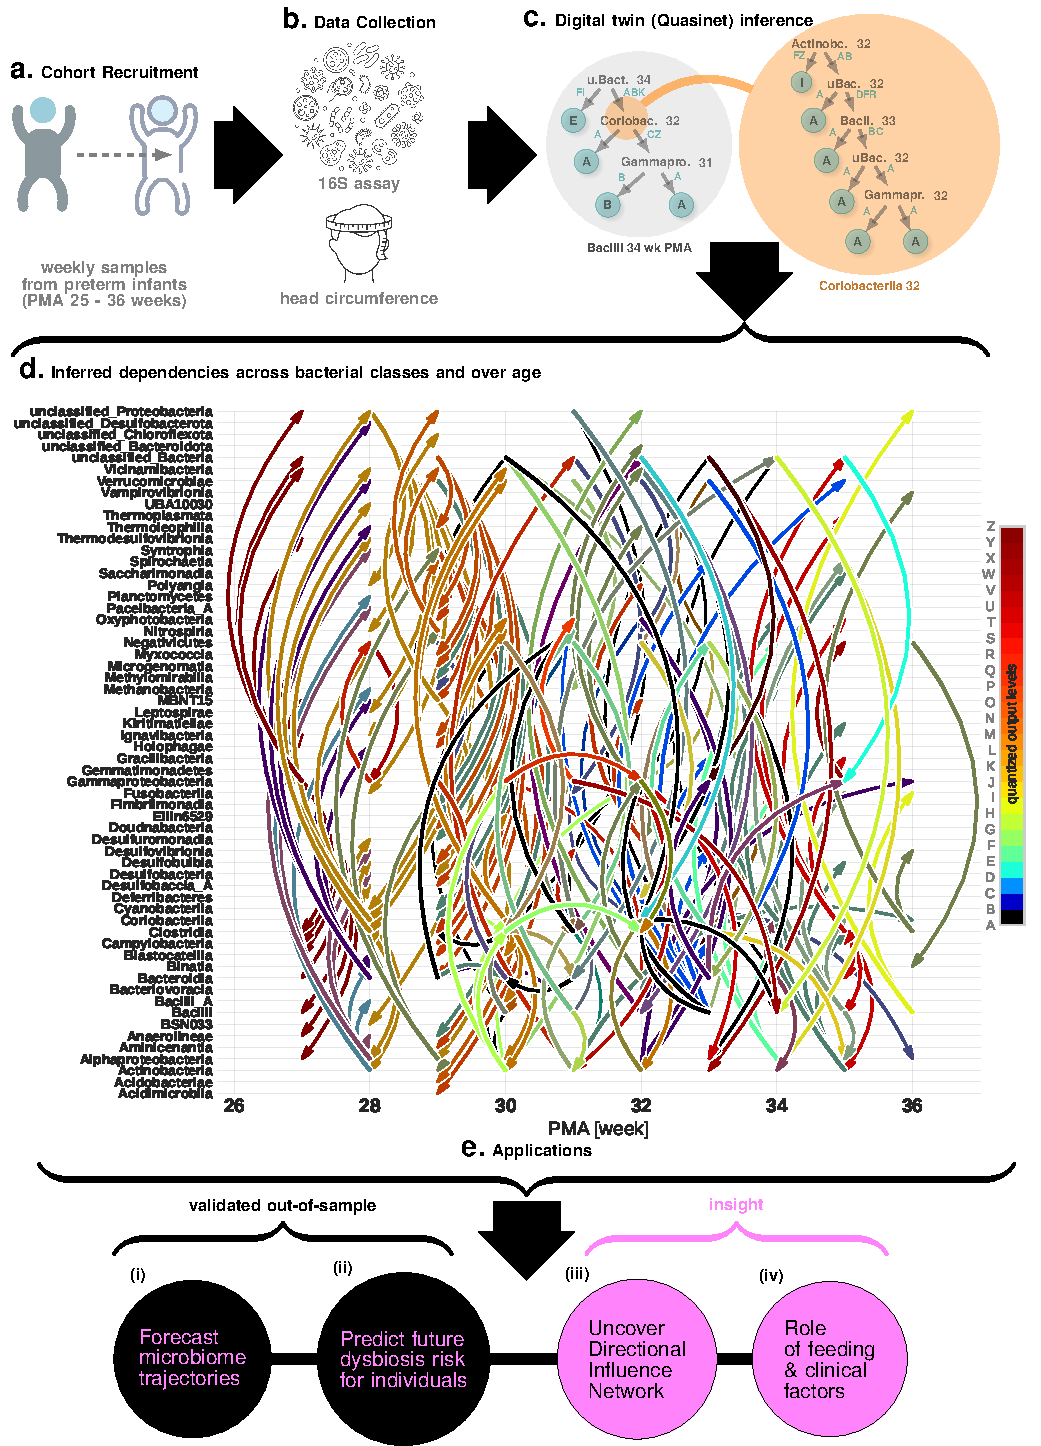
\includegraphics[width=0.8\textwidth]{fig1.pdf}
\captionN{\textbf{Scheme of study}. a-b, Longitudinal fecal samples from infants
born $<35$ weeks PMA  subjected
to 16S rRNA gene sequencing, along with infant head circumference growth (HCG) measurement. c, Microbiome abundance data is quantized into 26 levels between measured maxima for each observed taxonomic class, and is used to infer a digital twin, reflecting complex emergent dependencies across the classes via learning  a recursive forest of  conditional inference trees (the \qnet). Component trees in the \qnet (two examples shown) are inter-dependent, where  non-leaf node can recursively expand to its own tree. d, Complex dependencies inferred for typically developing sub-cohort across classes and observation time points. Each inferred dependency rule probabilistically relates an a priori unspecified number of entities ($>2$), and together specify a generative model of ecosystem trajectory and its dynamical operation. e, Applications enabled by the inferred digital twin, with out-of-sample validation and important mechanistic insights. }\label{figscheme}
\end{figure} 

%###############################
\begin{table}[t]
\caption{Demographic and clinical characteristics of study subjects in MIND cohort}
\centering
\label{tbl:patients}
\begin{tabular}{@{}p{6cm}S[table-format=3.2,round-mode=places,round-precision=4]S[table-format=3.2,round-mode=places,round-precision=4]S[table-format=3.2,round-mode=places,round-precision=4]S[table-format=3.2,round-mode=places,round-precision=4]@{}}
\toprule
\multicolumn{1}{c}{Characteristic} & \multicolumn{4}{c}{Description} \\
\cmidrule(lr){1-1} \cmidrule(lr){2-5}
Clinical target variable & \multicolumn{4}{c}{infant's head circumference growth (HCG)} \\
Clinical cohorts (2)                 & \multicolumn{4}{c}{appropriate HCG vs. suboptimal HCG}                \\
Patient age range                  & \multicolumn{4}{c}{$24$-$36$ weeks postmenstrual age (PMA)}                \\
Frequency of data collection                  & \multicolumn{4}{c}{$\approx$ weekly}                \\
Unique microbial phyla                  & \multicolumn{4}{c}{$44$}               \\
Unique microbial classes                  & \multicolumn{4}{c}{$91$}            \\[12pt]
%----------------------%
\multicolumn{1}{c}{Characteristic} & \multicolumn{2}{c}{UChicago} & \multicolumn{2}{c}{Boston} \\
\cmidrule(lr){1-1} \cmidrule(lr){2-3} \cmidrule(lr){4-5}
Number of patients                  & \multicolumn{2}{c}{$58$}    & \multicolumn{2}{c}{$30$}            \\

Avg. fecal samples/patient                  & \multicolumn{2}{c}{$4.13$}    & \multicolumn{2}{c}{$5.27$}              \\[12pt]
%----------------------%
& \multicolumn{2}{c}{UChicago}    &   \multicolumn{2}{c}{Boston}         \\
\cmidrule(lr){2-3} \cmidrule(lr){4-5}
                                    & {AHCG ($n = 28$)}    & {SHCG ($n = 30$)} & {AHCG ($n = 18$)}    & {SHCG ($n = 12$)}   \\
\cmidrule(lr){2-2} \cmidrule(lr){3-3} \cmidrule(lr){4-4} \cmidrule(lr){5-5}
\hangindent=2em Gestational age at birth (weeks), mean $\pm$ SD         & {$28.32 \pm 2.60$}    & {$26.9 \pm 2.64$} &  {$29.78 \pm 2.82$} & {$29.333 \pm 2.99$}  \\
Male, no. (\%)                      & {$13 \ (46.43\%) $ }     & {$15 \ (50\%) $ }    &  {$9 \ (50\%) $ }     & {$6 \ (50\%) $ }  \\
Birth weight, g, mean $\pm$ SD                   & {$1021.96 \pm 382.91$}  & {$998.3 \pm 423.45$} & {$1328.89 \pm 394.77$}  & {$1488.33 \pm 632.74$}\\
\hangindent=2em Birth head circumference, cm, mean $\pm$ SD                 & {$24.875 \pm 2.88$}  &  {$24.57 \pm 3.26$}  & {$27.32 \pm 2.22$}  &  {$28.25 \pm 3.27$}\\
Vaginal delivery, no. (\%)          & {$12 \ (42.86\%) $}   &  {$4 \ (13.33\%) $ }   &  {$6 \ (33.33\%) $}   &  {$4 \ (33.33\%) $ } \\
Length of NICU stay, days, mean $\pm$ SD    & {$77.89 \pm 34.77$} &   {$103.27 \pm 61.21$} & {$66.13 \pm 27.94$} &   {$72.09 \pm 33.61$}\\
\hangindent=2em Postmenstrual age at NICU discharge, weeks, mean $\pm$ SD & {$39.04 \pm 3.80$} &    {$41.13 \pm 6.80$} & {$39.33 \pm 2.09$} &    {$39.27 \pm 2.94$} \\[12pt]
%----------------------%
& \multicolumn{2}{c}{UChicago}    &   \multicolumn{2}{c}{Boston}         \\
\cmidrule(lr){2-3} \cmidrule(lr){4-5}
  \multicolumn{1}{c}{Microbial class (mean rel. abund.)}                                  & {AHCG ($n = 28$)}     & {SHCG ($n = 30$)} & {AHCG ($n = 18$)}     & {SHCG ($n = 12$)}    \\
 \cmidrule(lr){1-1} \cmidrule(lr){2-2} \cmidrule(lr){3-3} \cmidrule(lr){4-4} \cmidrule(lr){5-5}
Gammaproteobacteria & 0.647963 & 0.505579 & 0.650564 & 0.519976 \\
unclassified\_Bacteria & 0.076359 & 0.149064 & 0.067438 & 0.077718 \\
Clostridia & 0.073411 & 0.033252 & 0.027653 & 0.128344 \\
Bacteroidia & 0.063502 & 0.009749 & 0.018662 & 0.053227 \\
Bacilli & 0.046029 & 0.174091 & 0.123372 & 0.127355 \\
Negativicutes & 0.036066 & 0.044133 & 0.069160 & 0.045433 \\
Actinobacteria & 0.027100 & 0.031281 & 0.035964 & 0.037978 \\
unclassified\_Proteobacteria & 0.009649 & 0.040266 & 0.000010 & 0.000083 \\
Alphaproteobacteria & 0.007616 & 0.003534 & 0.002703 & 0.001581 \\
Fusobacteriia & 0.006863 & 0.003711 & 0.001340 & 0.005913 \\
Verrucomicrobiae & 0.000532 & 0.000810 & 0.000117 & 0.000158 \\
Vicinamibacteria & 0.000491 & 0.000901 & 0.000547 & 0.000402 \\
Nitrospiria & 0.000196 & 0.000364 & 0.000159 & 0.000169 \\
Oxyphotobacteria & 0.000144 & 0.000051 & 0.000024 & 0.000074 \\
\bottomrule
\end{tabular}
\end{table}
%###############################
    
\begin{figure}[!ht]   
\centering 
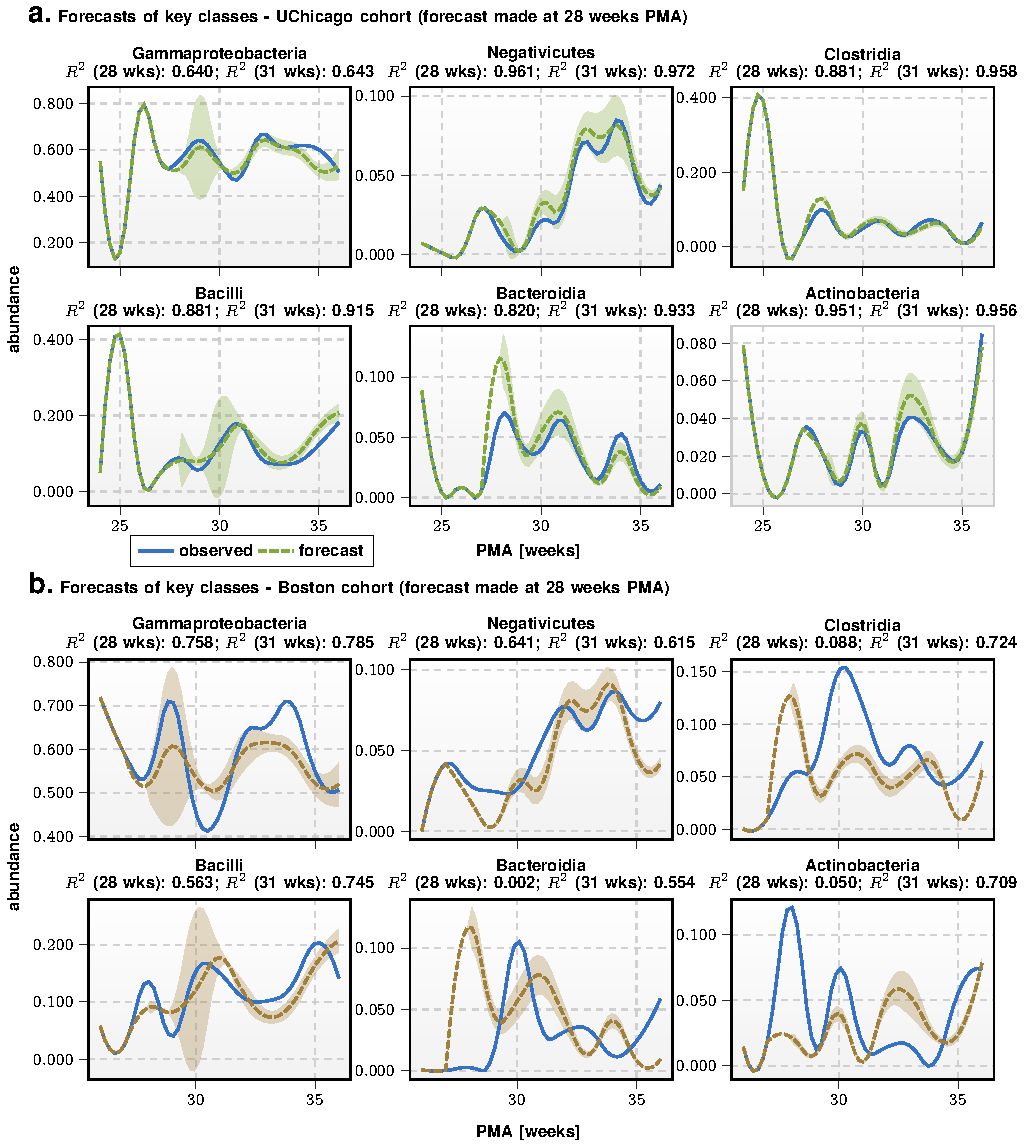
\includegraphics[width=.975\textwidth]{fig2.pdf}
\captionN{\textbf{Trajectory forecasts}. Population-level forecasting of mean abundance trajectories of select taxonomic classes (defined by having mean relative abundance $> 0.01$ in the training set) from a set of observations restricted to $<28$ weeks PMA. a, Forecasts generated from initial conditions specified by the UChicago cohort (from which the \qnet was inferred). Average $R^2$ across these taxa is $\approx 0.856$ at $28$ weeks, and $\approx 0.896$ at $31$ weeks. b, Forecasts generated using initial conditions specified by the Boston cohort (fully out-of-sample data which was not used for inference).  Average $R^2$ across these taxa is $\approx 0.350$ (which increases to $\approx 0.378$ when allowing for a temporal shift of $1$ week) at $28$ weeks, and $\approx 0.689$ at $31$ weeks.  In both cases, explained variance is typically high in these important classes, suggesting that the \qnet model successfully captures the complicated dynamical trajectories.   }\label{fig:forecast}
\end{figure}

%###############################
%###############################
\begin{figure}[!ht]
\centering
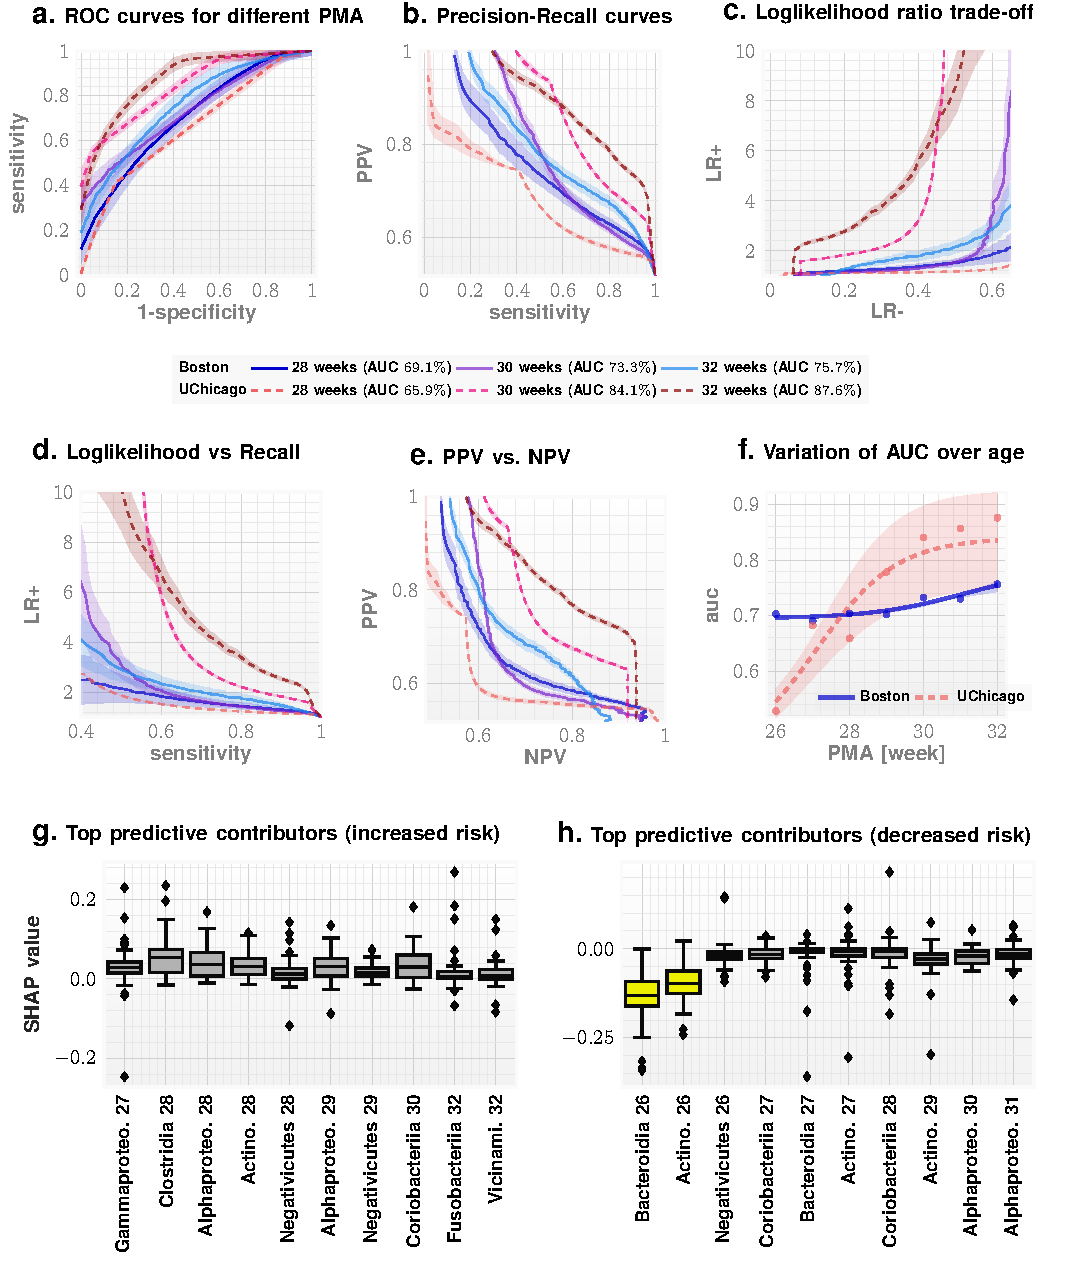
\includegraphics[width=.99\textwidth]{fig3.pdf}
\captionN{\textbf{Classification performance  out-of-sample}. a, Classification performance to recognize infants with eventually suboptimal HCG. The AUC is maximum at 32 weeks PMA reaching $87.6\%$ for the UChicago cohort (in-sample data), and $75.9\%$ for the Boston cohort. b, Precision-recall curves. c, Trade-off between positive (LR+) and negative (LR-) likelihood ratios. d, Change in LR+ with sensitivity or recall. e, Comparison of PPV vs. NPV at different PMA weeks. f, Fitting the computed AUCs over time, we note that the AUC $>80\%$ stabilizes approximately over 30 weeks PMA for the UChicago cohort. g, Top positive SHAP values for the \erisk risk driving HCG classification at 36 weeks PMA, and h, Top negative SHAP values for risk. Positive (negative) SHAP values indicate if an individual's abundance of a specific entity increases (decreases) the risk (compared to baseline samples) of a positive diagnosis of the target disease; thus the observed levels of Gammaproteobacteria and Clostridia (among others) are often associated with increased individual risk while Bacteriodia and Actinobacteria (among others) is similarly implicated with decreased risk. Note however that several taxa appear on both lists, suggesting complex dependencies of risk on entity abundances that vary over time.}\label{fig:perf}
\end{figure}

% #############################################
\def\HCOL{Green3!50}
\begin{table}[t]
\centering
\caption{Performance measures for classification at 30 weeks PMA}
\label{tbl:performance_chi30}

\begin{tabular}{lllllll}
\toprule
\multicolumn{7}{c}{UChicago}\\
\midrule
   fpr &               tpr &               ppv &               acc &               npv &                LR+ &               LR- \\
\midrule
$0.02$ & $0.466 \pm 0.015$ & $0.961 \pm 0.009$ & $0.714 \pm 0.008$ & $0.633 \pm 0.004$ & $23.288 \pm 0.767$ & $0.545 \pm 0.016$ \\
$0.04$ & $0.541 \pm 0.031$ & $0.935 \pm 0.009$ & $0.743 \pm 0.016$ &  $0.661 \pm 0.01$ & $13.516 \pm 0.773$ & $0.479 \pm 0.032$ \\
$0.06$ &  $0.56 \pm 0.033$ &  $0.909 \pm 0.01$ & $0.743 \pm 0.017$ & $0.666 \pm 0.013$ &   $9.328 \pm 0.55$ & $0.468 \pm 0.035$ \\
$0.08$ & $0.582 \pm 0.029$ & $0.886 \pm 0.009$ & $0.745 \pm 0.015$ & $0.672 \pm 0.011$ &   $7.27 \pm 0.357$ & $0.455 \pm 0.031$ \\
 $0.1$ & $0.598 \pm 0.021$ & $0.865 \pm 0.007$ & $0.744 \pm 0.011$ & $0.676 \pm 0.008$ &  $5.981 \pm 0.206$ & $0.447 \pm 0.023$ \\
$0.12$ & $0.614 \pm 0.021$ & $0.846 \pm 0.007$ & $0.742 \pm 0.011$ &  $0.68 \pm 0.009$ &  $5.116 \pm 0.173$ & $0.439 \pm 0.024$ \\
$0.14$ &   $0.63 \pm 0.02$ & $0.828 \pm 0.007$ & $0.741 \pm 0.011$ & $0.684 \pm 0.009$ &  $4.498 \pm 0.146$ & $0.431 \pm 0.024$ \\
$0.16$ & $0.645 \pm 0.021$ & $0.812 \pm 0.007$ & $0.739 \pm 0.011$ & $0.688 \pm 0.009$ &  $4.032 \pm 0.134$ & $0.422 \pm 0.026$ \\
$0.18$ &  $0.66 \pm 0.021$ & $0.797 \pm 0.007$ & $0.737 \pm 0.011$ &  $0.692 \pm 0.01$ &  $3.665 \pm 0.117$ & $0.415 \pm 0.026$ \\
 $0.2$ & $0.675 \pm 0.023$ & $0.784 \pm 0.007$ & $0.735 \pm 0.012$ & $0.697 \pm 0.011$ &  $3.376 \pm 0.114$ & $0.406 \pm 0.028$ \\
\midrule
\multicolumn{7}{c}{Boston}\\
\midrule
   fpr &               tpr &               ppv &               acc &               npv &                LR+ &               LR- \\
\midrule
$0.02$ & $0.345 \pm 0.181$ &  $0.95 \pm 0.018$ & $0.651 \pm 0.094$ & $0.586 \pm 0.069$ & $17.231 \pm 9.072$ & $0.669 \pm 0.185$ \\
$0.04$ & $0.367 \pm 0.166$ &  $0.916 \pm 0.02$ & $0.653 \pm 0.086$ & $0.589 \pm 0.065$ &  $9.163 \pm 4.156$ &  $0.66 \pm 0.173$ \\
$0.06$ & $0.395 \pm 0.145$ &  $0.887 \pm 0.02$ & $0.658 \pm 0.075$ & $0.595 \pm 0.059$ &  $6.588 \pm 2.409$ & $0.643 \pm 0.154$ \\
$0.08$ & $0.418 \pm 0.124$ &  $0.862 \pm 0.02$ &  $0.66 \pm 0.064$ & $0.598 \pm 0.052$ &   $5.221 \pm 1.55$ & $0.633 \pm 0.135$ \\
 $0.1$ & $0.441 \pm 0.116$ & $0.841 \pm 0.019$ &  $0.662 \pm 0.06$ &  $0.602 \pm 0.05$ &  $4.406 \pm 1.165$ & $0.622 \pm 0.129$ \\
$0.12$ &    $0.47 \pm 0.1$ & $0.821 \pm 0.019$ & $0.668 \pm 0.052$ & $0.609 \pm 0.046$ &  $3.917 \pm 0.837$ & $0.602 \pm 0.114$ \\
$0.14$ & $0.483 \pm 0.094$ & $0.802 \pm 0.018$ & $0.665 \pm 0.049$ &  $0.61 \pm 0.044$ &  $3.448 \pm 0.671$ & $0.601 \pm 0.109$ \\
$0.16$ &   $0.5 \pm 0.089$ & $0.785 \pm 0.016$ & $0.664 \pm 0.046$ & $0.612 \pm 0.042$ &  $3.123 \pm 0.555$ & $0.596 \pm 0.106$ \\
$0.18$ & $0.516 \pm 0.079$ &  $0.77 \pm 0.015$ & $0.663 \pm 0.041$ & $0.614 \pm 0.039$ &  $2.868 \pm 0.438$ &  $0.59 \pm 0.096$ \\
 $0.2$ & $0.532 \pm 0.078$ & $0.756 \pm 0.016$ &  $0.661 \pm 0.04$ &  $0.616 \pm 0.04$ &  $2.661 \pm 0.391$ & $0.585 \pm 0.098$ \\
\bottomrule
\end{tabular}



\end{table}
% #############################################

\begin{figure}[!ht]
\centering
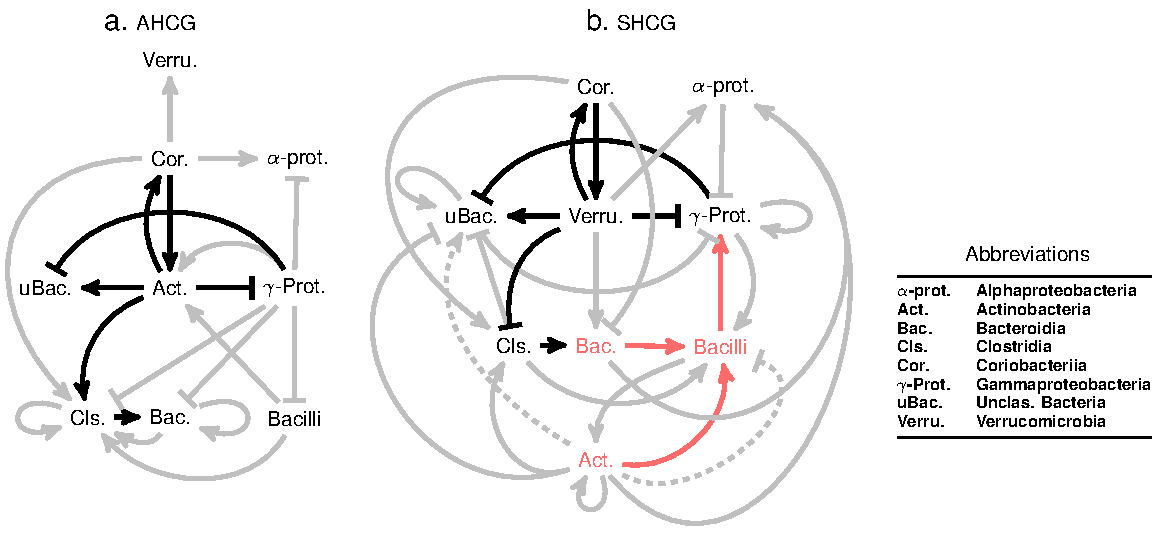
\includegraphics[width=.99\textwidth]{fig4.pdf}
\captionN{\textbf{Network structure comparison between typical and sub-optimal cohorts.} Change in inferred directional dependencies between prominent taxa in early development ($\leqq 31$ weeks) between optimal and sub-optimal head circumference growth, visualized via computing LOMAR coefficients. a, AHCG to b, SHCG. The bold edges highlight some key structural changes in \actn interactions. The edges in red show the key changes in \actn or \bact are supplanted as potential interventions in sub-optimal HCG. Dashed edges for \actn are interactions that emerge later than their corresponding non-dashed ones (\EXTENDEDDATA Tables~\ref{tbl:network_edges_ahcg_1},\ref{tbl:network_edges_ahcg_2},\ref{tbl:network_edges_shcg_1},\ref{tbl:network_edges_shcg_2}). Notably, SHCG interactions are both more complex and strongly connected.}
\label{fig:network}
\end{figure}

\begin{figure}[!ht]
\centering   
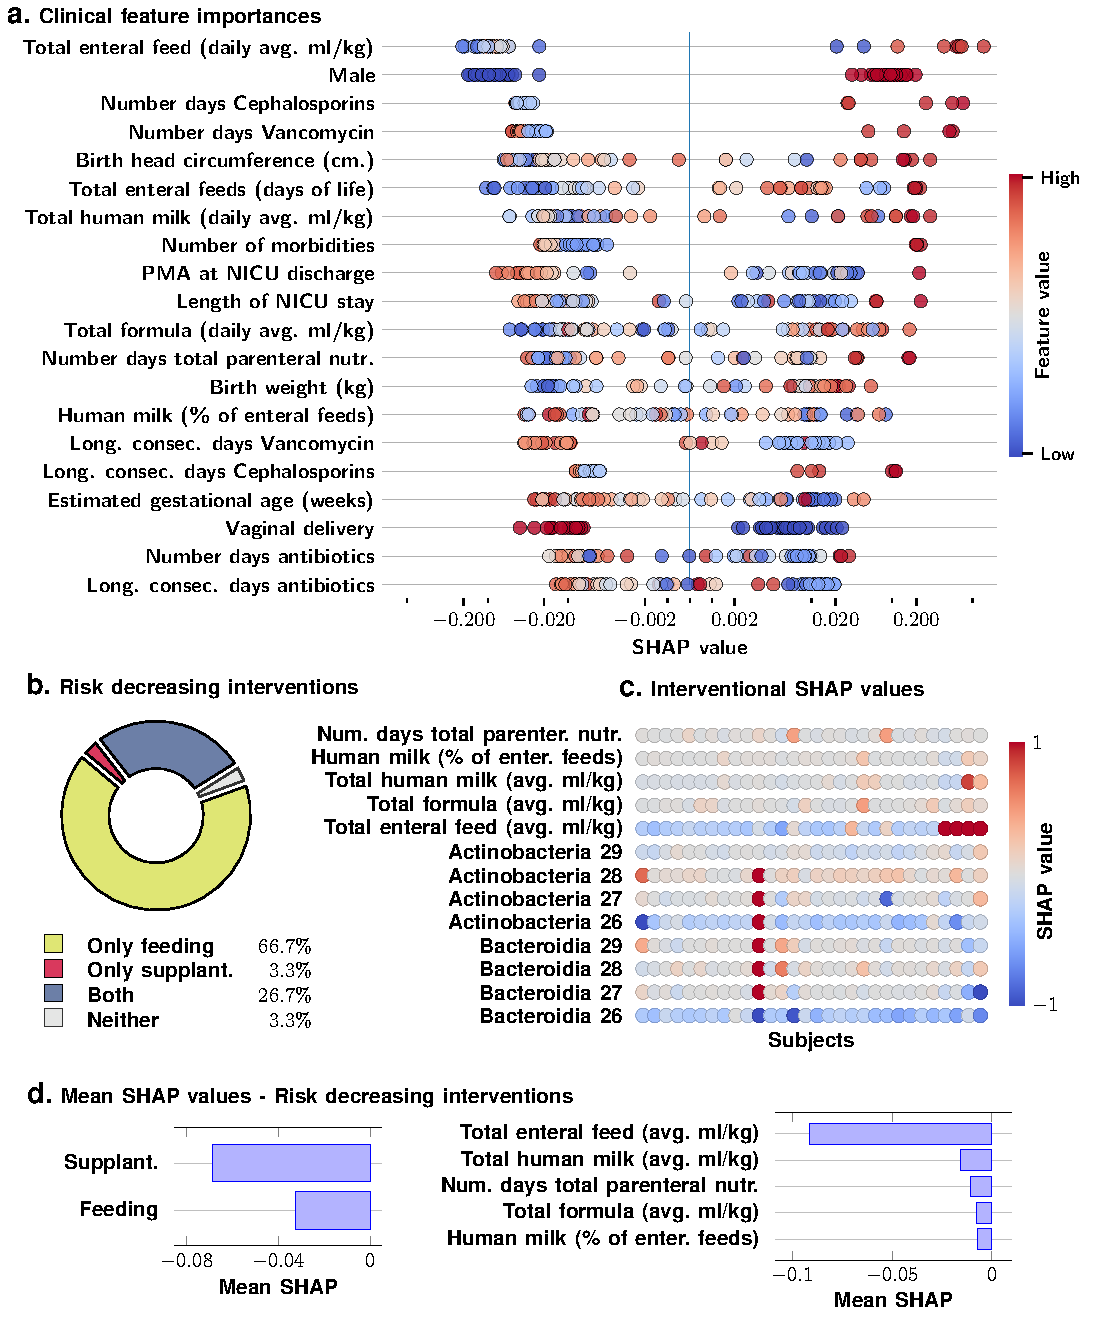
\includegraphics[width=.99\textwidth]{fig5.pdf}

\captionN{\textbf{Impact of clinical variables and diet}.  a,  impact  on \erisk risk of suboptimal HCG. We find that on average, being male, use of antibiotics, and enteral feed in amount and number of days maximally increase such risk. Panel b shows the distribution of SHCG patients by the types of intervention found to decrease their risk (microbiome-based supplantation intervention and/or feeding-based intervention).  Panel c depicts SHAP values for variables defining feeding and supplantation interventional categories in the SHCG cohort. Panel d shows that supplantation features are associated with greater decreases in risk than feeding, but that among feeding interventions, total enteral feed is associated with the maximum decrease in risk.}\label{fig:clinical}
\end{figure}
%###############################

\begin{figure}[!ht]  
\centering
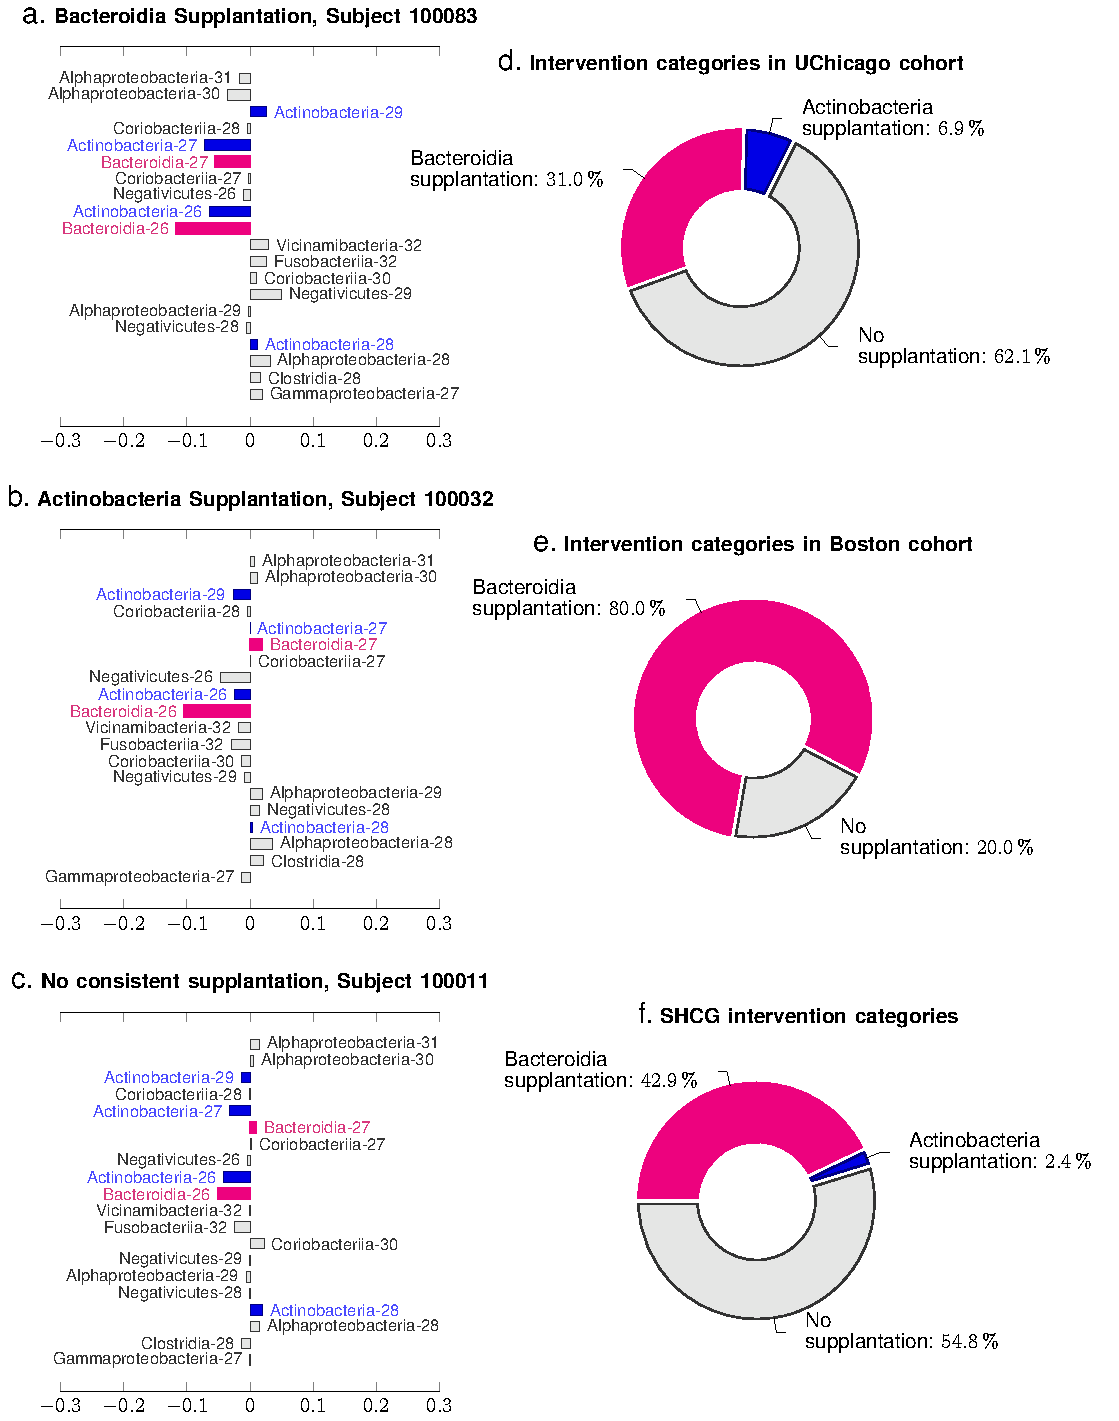
\includegraphics[width=\textwidth]{fig6.pdf}
\captionN{\textbf{Design of personalized early interventions to reduce risk of sub-optimal HCG}. a-c, SHAP profiles of three patients who have suboptimal HCG, but have three distinct intervention phenotypes, namely where supplnating \bact reduces risk (panel a), supplanting \actn reduces risk (panel b) and where no time-independent consistent supplantation can be obtained from our SHAP analysis (panel c). Both \actn and \bact have opposing effects on risk at different time points. d-e, the breakdown of these three intervention phenotypes in UChicago and Boston cohorts. f, breakdown of intervention phenotypes among all patients with sub-optimal HCG, showing that 45.2\% of patients have discernible interventions.  }\label{fig:shapphn}
\end{figure}
%###############################






In this study, we hypothesize that to delineate the impact of gut microbiome maturation trajectories on   cognitive development (assessed via the well-established proxy of head circumference growth~\cite{raghuram2017head,kuban2009developmental,neubauer2016poor,cordova2020association,hack1991effect}~\cite{belfort2007infant,oliphant2021bacteroidota}) in preterm infants, a  more profound understanding of the underlying rules of microbial organization is essential. To achieve this goal, we developed a computational framework that learns $n$-way time-aware dependencies among ecosystem inhabitants without imposing any a priori restrictions on the nature of interactions. This framework creates a digital twin of the ecosystem at the level of microbial classes for this case study (although any taxonomic level can be modeled). In engineering design, a digital twin represents a complex system comprehensively and accurately in a digital form, enabling the simulation of perturbations, study of trajectories, aberrations, and failures, and the execution of high-fidelity simulation experiments that would otherwise be unattainable in the real world. Rather than answering a single question, a digital twin aims to mirror the entire system, distinguishing it from typically more limited standard  machine learning models.

We found that our digital twin, which we refer to as the \qnet, successfully generates reliable long-term forecasts of coupled trajectories for key microbial classes in realistic patient populations. Furthermore, it unveils meaningful patterns that increase the risk of future suboptimal cognitive development. The detailed dependencies across bacterial classes that we identify provide interpretable insights unattainable through a standard predictive model alone. In contrast to existing methods, our digital twins serve more than just a forecasting function; we explicitly use them to determine patient-specific risk measures that can be assessed early enough to design targeted clinical interventions, validated out-of-sample from a second independent study site.


\section*{Results} 
\subsection*{Data Source}
Our first data source comes from a cohort of $58$ preterm infants born less than $35$ weeks gestational age, recruited~\cite{oliphant2021bacteroidota} from University of Chicago's Comer Children's Hospital to join the  Microbiome in Neonatal Development (MIND) study, referred to as the UChicago cohort.  This dataset consists of longitudinal fecal samples of microbial relative abundances obtained from the subjects via 16S rRNA gene sequencing~\cite{walters2016improved,caporaso2012ultra} measured weekly from birth to term-equivalent age for each patient ($24$-$36$ weeks postmenstrual age (PMA), See \SUPPLEMENTARY Fig.~\SPREFIX\ref{fig:violin} for a mapping between weeks of life and PMA), as well as a variety of clinical variables such as delivery mode, feeding type, antibiotic usage, etc (See Fig.~\ref{figscheme} for overall scheme of the study). Technical details of sequencing and data processing described in \cite{oliphant2021bacteroidota} are also given in \Methods~ Section \ref{sec:data_src_proc} and descriptions of the variables measured in the study are enumerated in \SUPPLEMENTARY Table~\SPREFIX\ref{tbl:clinical_vars}. 

For out-of-sample validation, a second cohort of $30$ preterm infants born less than $35$ weeks gestational age from the MIND study were recruited at the Beth Israel Deaconess Medical Center, Boston, Massachusetts (referred to as the Boston cohort). For both cohorts, we target a clinical response of the classification of patients by level of cognitive development reflected by the proxy of head circumference growth (HCG), which is assessed here via difference in head circumference $z$-score from birth to term-equivalent age ($36$ weeks postmenstrual age) to the Fenton growth curve~\cite{fenton2013systematic,cordova2020association}. 

We consider two clinical phenotypes~\cite{oliphant2021bacteroidota}: infants who ultimately attain appropriate ($\geq -0.5$ $z$-score difference) vs suboptimal ($< -0.5$ $z$-score difference) head circumference growth (AHCG, SHCG respectively).  Overall patient characteristics are presented in Table~\ref{tbl:patients}. Notably, the phenotype distribution of the UChicago cohort was nearly balanced, with $28$ infants classified as AHCG and $30$ SHCG; similarly, it was nearly balanced with respect to sex distribution, the cohort contained $30$ females and $28$ males. Similarly, the Boston cohort also had a relatively balanced distribution of $18$ infants with AHCG and $12$ infants with SHCG, and an equal male/female ratio.  With respect to the observed taxonomy, across both cohorts, samples contained microbial entities from $44$ unique phyla and $91$ distinct classes. Table \ref{tbl:patients} contains a listing of the most abundant entities by class in separate subcohorts induced by head circumference growth classification; notably $\approx 10$ entities are sufficient to capture $99\%$ of mean relative abundance.

We chose to obtain our generative model at the taxonomic level of microbial classes. To address the compositional nature of relative abundance data, we quantize all observations into a finite number of bins corresponding to quantiles of the range of relative abundance values recorded over the entire time period for the specific microbial class.  Our model  operates on these quantized observations; for subsequent interpretation we map relevant quantized values back to continuous relative abundances (See \Methods, Section~\ref{sec:qnet_constr}). 

\subsection*{Digital Twin Construction from Longitudinal Microbiome Profiles}
We construct our models using the relative abundance profiles observed in the UChicago cohort, and carryout out-of-sample validation of these models for doing long-term forecast of microbiome maturation, as well as predicting the risk of suboptimal developmental outcomes in the Boston cohort. The different digital twins produced in this study are represented in  \SUPPLEMENTARY Table~\SPREFIX\ref{tbl:models_links}. Note that \qnet inference algorithm is not deterministic, and inferred models exhibit small variance with respect to connections and generative probabilities. Thus to ensure robustness/validity, our results are based on an ensemble of models generated by re-fitting multiple times on the same underlying data (See \Methods, Section~\ref{sec:regen}).

Relative abundances of the microbes vary under emergent constraints of competition, amensalism, cooperation, commensalism and exploitation, and many of these dependencies  are unknown or poorly understood a priori.  From the observed time-stamped samples of microbiome profiles, we aim to maximally infer these complex rules (Section~\ref{sec:qnet_constr} in \Methods) as follows. For each patient, we treat observed relative abundances of each microbial class at a specific time-point (identified by the PMA of the subject at the time of sample collection) as a  distinct variable or ``feature''. The \qnet, inferred from this data, consists of a set of distinct predictors, each modeling the  expected probability distribution of the relative abundance of a specific  variable (a microbial class at a specified timepoint, or a class-timepoint pair), conditioned on  the remaining variables, $i.e.$, the rest of the microbial relative abundances recorded possibly at different time points. Importantly, no locality restrictions on temporal dependence are made, and the model is free to infer  dependencies present between different entities across all past time points. Thus, we may have as many estimators as the number of observed microbial classes times the number of discrete time-stamps, $i.e.$, for our data set: $91$ classes $\times 12$ time points $= 1092$ (although not all classes had non-zero observations at all time points).


In each \qnet, we infer our component predictors described above as  conditional inference trees~\cite{hothorn2006unbiased,sarda2017conditional}, which use explicit statistical tests to ensure that each node-split during the tree construction is significant at a preset level, and thus limits over-fitting. Each of these decision trees aims to predict the relative abundance level of a specific bactaerial class at a specific timepoint,  and uses as features other bacterial classes similarly coupled with corresponding time-stamps. A fragment of a \qnet is shown in Fig.~\ref{figscheme}c, where the predictor for Bacilli at 34 weeks PMA is shown on the right, which uses as features ``Unclassified Bacteria at 34 weeks'', ``Coriobacteriia at 32 weeks'' and ``Gammaproteobacteria at 31 weeks'' as predictive features, \textit{i.e.}, these are the variables that appear in the internal nodes of the tree. Note that the feature ``Coriobacteriia at 32 weeks''  has its own predictor as shown on the right, and  uses as features ``Actinobacteria at 32 weeks'', ``Unclassified Bacteria at 32 weeks'', ``Bacilli at 33 weeks'', and ``Gammaproteobacteria at 32 weeks''. Thus, any non-terminal node of a component tree for an inferred \qnet can in general be ``expanded`` to its own tree. Owing to this recursive expansion,  a complete \qnet is difficult to visualize simultaneously, but it nevertheless substantially captures the complexity of the  rules shaping  the ecosystem as evidenced by our out-of-sample validation.  (Note that there is always imprecision with regards to the timing of these events, partly due to the possibility of $\approx 1-2$ week   ambiguity in post-menstrual age of the infants, and hence we consider features timestamped to be in future by upto 2 weeks to impact an entity. This ``flexibility'' is only allowed in the inference stage and not in testing, and thus do not affect prediction results.) The set of features that a particular estimator uses is identified automatically, and the inferred ensemble of conditional inference  trees  maximally captures the organizational structures emergent in the observed microbiome profiles. The rich tapestry of multi-way time-aware cross-talk that we infer is depicted in Fig.~\ref{figscheme}d.

With our inferred models, we carried out five computational interrogations, namely i) forecasting microbiome maturation trajectories for out-of-sample subjects, with very few initial observations, ii) out-of-sample  prediction of  the phenotypic fate of infants with regards to their cognitive development from their forecasted microbiome maturation trajectories to evaluate the relative risk of suboptimal development at a time point early enough for potential intervention, iii) uncovering a directional influence network connecting the observed taxa, to determine critical ecosystem constituents that differentiate phenotype from both their relative influence on microbiome maturation trajectories and changes in network connectivity at each time point, a concept that moves beyond defining important taxa through changes in relative abundance towards their relative role in ecosystem dynamics over time, iv) interrogating the role of key clinical factors in shaping  microbiome maturation and dysbiosis over time (Fig.~\ref{figscheme}e) and v) determining microbiome or clinical interventions that could reduce risk of SHCG on a personalized level. Reasoning with the patterns that the \qnet inferred is made possible via two key computations: 1) sampling the digital twin to impute missing data in a manner that obeys the inferred probabilistic constraints, and 2) quantitatively assess the dissimilarity of two distinct  microbiome trajectories, via  an  intrinsic distance  induced by the \qnet model. Here a ``microbiome trajectory'' refers to time-stamped relative abundance values of all observed microbial classes, possibly with  missing entries. 
%
\subsection*{Sampling the Digital Twin For Imputation and Forecasting}
The inferred \qnet allows us to impute missing relative abundance values that maximally exploit the learned dependencies across taxa. Our procedure  is conceptually equivalent  to the well-known Gibbs sampling scheme~\cite{geman1984stochastic,casella1992explaining}. We can  estimate the  missing relative abundance value of a specific bacterial class at a given time, by drawing a sample from the conditional distribution for the corresponding variable $i.e.$ a class-timestamp pair, as estimated by the \qnet. As is the case for  Gibbs sampling, if repeated such samples are being drawn, in the limit we are  sampling from  the joint distribution of all variables, $i.e.$,  the space of all feasible microbiome trajectories. We use this imputation scheme  to forecast maturation dynamics: fixing a set of initial conditions corresponding to all observed relative abundances at times $t < 28$ weeks PMA, we treat future relative abundances from $28$ weeks PMA and later as unknown or missing,  which we can then impute iteratively, with the new values obtained essentially being the predicted relative abundances. 

\subsection*{Validation and Comparison of Forecast Performance for Microbiome Maturation Trajectories}
  We evaluate the quality of these predictions  by assessing the coefficient of determination or the R-squared measure ($R^2$) between observed mean relative abundance and model-predicted values from initial conditions specified by separate independent data sets prior to $28$ and $31$ weeks PMA.  We achieve average $R^2 > 0.85$ on forecasts of the UChicago cohort (in-sample) starting from $28$ weeks PMA and average $R^2 = 0.89$ for the $31$ weeks PMA forecasts. For the out-of-sample Boston cohort we achieve an average  $R^2 = 0.69$ at the $31$ weeks PMA prediction, while the results for out-of-sample prediction at $28$ weeks PMA are somewhat worse as expected (mean $R^2 = 0.35$). The results are shown in Fig.~\ref{fig:forecast}, with $95\%$ confidence bounds. It is important to note that if we allow relative shift between the predicted and observed time courses of $\pm 1$ week, then the mean $R^2 = 0.52$ for predictions at $28$ weeks (the prediction at $31$ weeks does not improve with this possibility of relative shifts), indicating some degree of uncertainty in PMA estimates of the infants, especially for those who are born earlier than 30 weeks. Increased challenge of determining PMA for early preterm births have been reported before~\cite{dietz2007comparison}.
 
To place these results in context, we compute  the coefficient of determination $R^2$ obtained by Dynamic Bayesian Networks (DBN), which represent the state of the art framework in longitudinal forecasting of relative abundances of microbial taxa. We implemented a direct comparison (see \Methods~Section \ref{sec:forecast} for details) of our \qnet-based approach to DBNs, exploring various level of DBN model complexity. These results are shown in \EXTENDEDDATA Figure~\ref{fig:baseline} and and \EXTENDEDDATA Table~\ref{tbl:baseline_comparisons}, which depict the forecasting performance of Dynamic Bayesian Networks (DBN) of increasing depth from 2-stage to 6-stage architectures on both the UChicago cohort (in-sample) and Bostn cohort (out-of-sample). Forecasts are made at $28$ and $31$ weeks PMA for all models; we found that all of the DBNs evaluated attained $R^2$ less than half of the corresponding \qnet-based approach. This substantial reduction in $R^2$ is demonstrative of a concurrent substantial reduction in the ability of DBNs to model this data in comparison to the \qnet approach.  


\subsection*{Quantifying Future Risk \erisk of Anomalous  Deviation  in Microbiome Maturation}
In our study, we recognize that the infant microbiome maturation trajectory is influenced by prominent stochastic components, with any observed trajectory being just one possible realization. Anomalous deviations from a typical maturation path aren't merely changes from the observed one, as multiple healthy trajectories might be feasible, 
and a precise characterization of all such typical trajectories is not known a priori. At the same time, we know that arbitrary perturbations to an observed profile might not be feasible, as evidenced by the challenges of making desired changes to a microbiome profile via various microbial manipulations~\cite{lopez2016fecal}. Qualitatively,  if two trajectories lead to healthy outcomes \textit{i.e.} are exchangeable, then we wish to identify them to be similar, whereas if one ultimately leads to poor  outcomes, then our aim here is to be able to recognize the increased clinically meaningful dissimilarity.

With the ability to learn digital twins separately for sub-cohorts corresponding to typical and suboptimal development respectively, we quantify clinically  meaningful similarity between two stable microbiome trajectories $\x,\y$ as  the odds of an observed  trajectory $\x$ being spontaneously replaced by another  $\y$  by random chance (which is plausible given that observed trajectories are sample paths from underlying stochastic processes). Thus, in our approach, the higher the probability $\operatorname{Pr}(\x \rightarrow \y)$ the more similar they are. We estimate $\operatorname{Pr}(\x \rightarrow \y)$ by crafting an intrinsic distance between  microbiome trajectories. The \qdist  $\theta(\x,\y)$ between two microbiome trajectories is defined (Definition~\ref{defqdistance} in \Methods) as the square-root of the Jensen-Shannon (JS) divergence~\cite{cover} of the conditional relative abundance distributions induced by the inferred \qnet for a  specific class at a  specific time, averaged over all class-timestamp pairs. We show from theoretical considerations (Theorem~\ref{thm:probbnd} in \Methods) that the \qdist  approximates the log-likelihood of  spontaneous change in the microbiome trajectories  $i.e.$ $\theta(\x,\y) \approx \textrm{constant} \times \log \operatorname{Pr}(\x \rightarrow \y)$. 

With this notion of the \qdist we can quantify  the risk \erisk of future anomalous deviation  for individual patients to address the following question: \textit{Given an observed current trajectory of a specific patient (typically with few initial observations), estimate their risk of developing with a cognitive deficit as opposed to proceeding with typical  development.} We estimate \erisk risk as the ratio of the log-likelihood of an observed trajectory $\x$ (for a given patient) being realized in the suboptimally developing cohort to the log-likelihood of the same trajectory being realized in a typically developing cohort. Thus, our risk estimate quantitatively assesses which of the two models explain the data observed so far for individual patients. To demonstrate the effectiveness of our risk measure, we  validate its ability to predict the HCG phenotype in out-of-sample data (the Boston cohort), where the two digital twins corresponding to the typical and suboptimal development $i.e.$ the AHCG and the SHCG cohorts, are constructed using the UChicago samples. 

\subsection*{Validation of \erisk Risk as a Measure of Future Sub-optimal Head Circumference Growth}
To validate our risk measure predicting future anomalous deviations, we set up a classification problem to predict the eventual HCG phenotype of individual patients. We found that classification based on the \erisk risk  yields significantly and substantially improved performance over naive baselines based on microbial relative abundances and clinical factors (baseline model: random forest), as described next. On the UChicago (training) cohort ($58$ patients, $158$ fecal samples, $18564$ abundance measurements), we achieve peak area under the receiver-operator characteristic curve (AUC) at $32$ weeks of $87.6\%$ (measured by out-of-bag score, a proxy for out-of-sample performance; performance achieved using the only \erisk risk; compared to median AUC $39.3\%$ for a baseline classifier trained using only delivery mode without the risk score; results at different weeks of prediction with additional clinical variables are shown in \SUPPLEMENTARY Table \ref{tbl:clin_var_comparisons}). At $80\%$ specificity, we achieve sensitivity of $75.9\%$, positive likelihood ratio of $3.79$, and negative likelihood ratio of $0.3$, while at $90\%$ specificity we achieve sensitivity $61.7\%$, positive likelihood ratio of $6.17$ and negative likelihood ratio of $0.43$.  On the Boston (validation) cohort ($30$ patients, $248$ fecal samples, $14378$ abundance measurements), we achieve peak AUC of $75.7\%$ (performance achieved using the \erisk risk and the clinical variables delivery mode, birth weight, birth head circumference, and estimated gestational age; compared to median AUC $62.4\%$ for a baseline classifier using the same clinical variables but without the risk score) with sensitivity $53.3\%$ at $80\%$ specificity, positive likelihood ratio of $2.67$ and negative likelihood ratio of $0.58$ (Fig.~\ref{fig:perf}a-f). We note that our inferred classifier may be operated with different choice of specificity vs sensitivity trade-offs. For example, we might choose to operate the model at the maximum achievable PPV at a  set value of the false positive rate. The variation of these performance measures at various possible operating points at 30 week PMA  is enumerated in Table~\ref{tbl:performance_chi30}, along with 95\% confidence bounds. We note that at 2\% false positive rate (98\% specificity), we achieve 95-96\% PPV, and a positive likelihood ratio $17.2 \pm 9$, which implies that for a patient flagged to be at high risk for developmental deficit, their risk is greater than 9 to 26 times that of the general population. Detailed performance at 32 weeks PMA is shown in \SUPPLEMENTARY Table\SPREFIX~\ref{tbl:performance_chi32}. The trade-offs between specificity and sensitivity obtained at different time points measured in weeks PMA is shown in Fig.~\ref{fig:perf}a. Panel b shows the trade-offs between positive predictive values (PPV) and sensitivity, and panel c shows the trade-offs between the positive and negative log-likelihood ratios. Panel f shows the  improvement of AUC with patient age, which is expected as more information is collected over time. 


\subsection*{Importance of Different Taxa In Determination of HCG Phenotype}
To investigate how specific bacterial classes modulate HCG, we  perform a Shapley Additive Explanation (SHAP) analysis~\cite{NIPS2017_7062,lundberg2018explainable}, a model-agnostic method of computing feature importances where the impact of each feature on the model is uncovered  using the game-theoretic Shapley values~\cite{vstrumbelj2014explaining,roth1988shapley}. The SHAP analysis (Figure~\ref{fig:perf}g-h) found that the top influencers (exerting both positive and negative influences)  are most impactful prior to $30$ weeks PMA as evidenced by the time-stamps of the top 10 risk increasers (panel g) and top 10 risk decreasers (panel h) which are between 28-31 weeks PMA. Here, by the standard interpretation of SHAP values, increasing the relative abundance of the microbial classes in panel g (with positive SHAP values) would increase the risk of a cognitive deficit (and thus these microbes are over-abundant at their corresponding observation times), while those in panel h (with negative SHAP values) would decrease risk if made more abundant, and are thus under-abundant at their corresponding time-stamps.
In particular, increasing  the $26$ weeks PMA levels of  \bact, and the $26$ weeks PMA levels of \actn will  decrease risk on average,  while increasing the $27$ weeks PMA levels of \gamm, and the $28$ weeks PMA levels of \clsd  will  increase risk on average. It is notable that the SHAP analysis finds some of the microbial taxa most contributive to risk $e.g.$ Negativicutes and Coriobacteriia,  exhibit an increasing affect on risk at one time point and a decreasing affect on risk at a different time point, suggesting that {\qnet}s are capable of capturing subtle variations in the key drivers of risk over time.  It is important to note that these average impacts to perturbations   are not recommendations that may be used for supplanting the microbiome, as we demonstrate later that such actions necessarily need to b personalized, and what is beneficial for one infant might be detrimental for another.

\subsection*{Network Analysis to Uncover Across-taxa Directional Influence on Abundunce Fluctuations}

 To better interpret the inherently asymmetric directional influences between taxa in the ecosystem, we  compute what we refer to as the Local Marginal Regulation (LOMAR) coefficient(s) for each pair of observed interacting bacterial classes. The LOMAR coefficients represent the up-regulatory/down-regulatory influence of a source taxonomic class on a target class, where regulation effects are causally localized in time (future cannot affect the past), and where potential confounding effects from other taxa are averaged out. Using this notion, we can inspect   the ``influence network''  recovered by the \qnet, allowing us to visualize the major differences between the digital twins inferred for the optimal and sub-optimal cohorts.

   After computing the set of LOMAR values for each model (see Section~\ref{sec:lomar} for details and \EXTENDEDDATA  Tables~\ref{tbl:network_edges_ahcg_1}-\ref{tbl:network_edges_shcg_2} for the computed LOMAR values), we plot the asymmetric relations as  directed graphs in Figure~\ref{fig:network}.  Comparing these networks in early stages of development (27-30 weeks PMA, Figure~\ref{fig:network}a-b), we see that the optimal and sub-optimal models are quite distinct, with different roles being played by \actn and \verru as hub nodes, and in general, the SHCG model has more interactions.

\subsection*{Role of Clinical Factors and  Diet In Modulating HCG Phenotypic Outcome}

To assess the importance of  clinical factors in modulating microbiome maturation trajectories, we carried out a SHAP analysis of a random forest regression model, with the \erisk risk as the dependent variable, and  all  available clinical factors as explanatory variables or features (Fig.~\ref{fig:clinical}).  We observe that factors such as longer time until total enteral feeding is achieved, sex being male,  the total number of morbidities, number of days on Cephalosporins, number of days on Vancomycin, lower gestational age at birth, and total formula in diet subtantially raises risk on average. Importantly, we found  vaginal  delivery (VD) as the only substantially risk-reducing factor, with a mild benefit from increasing the proportion of human milk in diet. We note that some factors which reduce risk on average increased risk for some participants and vice versa, suggesting the complex contextual impact of these environmental variables. One such example is the total amount of enteral feeds which highly increased risk of SHCG in a small subset of individuals. Nevertheless, male sex emerges as a key factor driving HCG outcomes.

\subsection*{Designing Personalized Interventions To Reduce Risk of Poor HCG Outcome}
The SHAP analysis of the digital twins inferred for the optimal and sub-optimal cohorts lays the foundation for designing early personalized interventions based on supplanting specific microbial taxa in infant diet. Importantly, note that a positive SHAP value of a variable (in this case, the relative abundance of a specific taxa at a specific time point) implies that increasing the value of the variable ($i.e.$ the relative abundance of the taxa in question at the particular timepoint associated with that variable) will increase risk on average, and vice versa. Also note that many of the bacterial taxa appear in both panels g and h of Fig.~\ref{fig:perf}, $i.e.$, based on the time-point they can be either risk increasing or risk-decreasing if their relative abundances are increased. However not all bacterial taxa have this time-dependent impact, and here we focus on microbial classes that have a consistent average negative SHAP value ($i.e.$ risk-decreasing impact) over time, to define effective interventions. Inspecting panel Fig.~\ref{fig:perf}h, we conclude that \bact and \actn are the only two taxa that are substantially and consistently risk decreasing on average, and early supplantation of these taxa is expected to reduce risk of sub-optimal outcomes in HCG.

As before, the average trend is not representative for every participant. Since the SHAP values are patient-specific (Fig.~\ref{fig:perf}g,h showing averaged values over the UChicago cohort),  we can use the notion of consistent impacts as defined above to deduce patient-specific interventions. Using this notion we end up identifying three intervention  phenotypes: a) Early \bact Supplantation, b) Early \actn Supplantation, and c) Null, or patients for whom  no such time-independent interventions can be found that would tend to reduce risk. Fig.~\ref{fig:shapphn}a-c illustrates specific patients in these three categories. We found that $31.04\%$ of the UChicago cohort fell into the \bact Supplantation category, with $6.9\%$ in the \actn category, and $62.07\%$ were in the Null category (Fig.~\ref{fig:shapphn}d). The corresponding numbers in the Boston category were $80\%$ amenable to \bact Supplantation, and the rest in the Null category (Fig.~\ref{fig:shapphn}e). Overall we found that considering all patients in the sub-optimally developing cohorts, $42.9\%$ would have had a risk reduction from early \bact supplantation, and $2.4\%$ from early \actn supplantation, while the remaining $54.8\%$ of the patients did not have any time-independent risk-reducing interventions (Fig.~\ref{fig:shapphn}f). Additionally we found that categories are mutually exclusive, implying that choosing the incorrect intervention could be counter-productive, increasing the risk of suboptimal HCG.

We also investigated such potential intervention designs using the modifiable factors that relate to diet. In particular we consider the impact of the amount of total enteral feed, total formula fed, total human milk fed, human milk fed as a percentage of total feed, and the number of days the subject received total parenteral nutrition. Examining the SHAP values for these factors (Fig.~\ref{fig:clinical}b,c), we find that the majority of patients ($94.4\%$) with suboptimal HCG have at least one negative SHAP value. Of these, $66.7\%$ do not have a supplantation intervention, while $26.7\%$ may respond to both feeding and supplantation interventions. Thus, our results suggest that most patients with suboptimal HCG may experience possible reduction in risk due to a subset of these specific feeding interventions.  While these dietary factors do not appear to have as strong of an effect as supplantation (mean SHAP value of $-0.06$ vs. $-0.03$ for risk decreasing supplantation samples compared to risk decreasing feeding samples), the feeding interventions are perhaps more broadly applicable. Amongst the feeding interventions, we find the greatest risk-decreasing effect from such interventions (on average) appears due to the amount of total enteral feed, which has mean SHAP of $-0.09$ compared to $\leq -0.01$ for each of the other variables. (Fig.~\ref{fig:clinical}d). Note however, that there is individual variation present (Fig.~\ref{fig:clinical}c) with some individuals appearing to have increased risk from this factor,  stressing the importance of a personalized, targeted approach to any interventional strategy.

%###########################################
%EXTRACT
\section*{Discussion}
Despite increasing evidence of  the critical role of the gut microbiome in pediatric health,  remaining challenges  in inferring  interactions across diverse microbial taxa obfuscates  identification of actionable colonization patterns that might foreshadow poor clinical outcomes. These limitations hinder the  design of   clinical interventions  in vulnerable populations, such as preterm infants, that might otherwise prove effective in  ameliorating developmental deficits.  Recent work demonstrating the connections between relative abundance of key microbiome taxa and cognitive development in preterm infants~\cite{oliphant2021bacteroidota} suggests that subtle  patterns in relative abundance data can provide actionable  clinical insights.  In this study, we work towards uncovering these connections via  a novel  machine learning approach to infer a generative detailed model of the developing ecosystem. Our model is structurally rich, allowing complex time-dependent patterns to emerge, yet sufficiently interpretable to be  clinically meaningful.   

Considering the problem of uncovering the role of gut microbiota of preterm infants in cognitive development, our key findings are as follows: 1) reliably forecast the coupled development of microbial communities for weeks from very limited initial observations, 2) obtain  clinically useful predictive performance (demonstrated through out-of-sample validation on an external cohort) for prediction of sub-optimal phenotypes of cognitive development from microbiome relative abundance profiles, 3)  identify statistically significant direction-specific relationships between entities within the maturing ecosystem, 4) investigate the relative importance of  prominent clinical factors and diet in modulating maturation trajectories, and  5) 
suggest principled approach to personalized early interventions that can reduce the risk of sub-optimal HCG.

These capabilities are enabled via  inferring complex temporal relationships amongst microbial classes without an a priori  fixed parametric structure. Instead of modeling the observed relative abundances to answer specific questions, we learn an approximate yet sufficiently detailed model of multi-way interactions in the ecosystem, yielding a digital twin that enables imputation of missing data, trajectory forecasts, and estimates of future risk of poor developmental outcomes. Additionally,  our explicit representation of temporal dependencies enables us to identify variations in predictive performance over time, which  provide insights into the timing of fundamental shifts in ecosystem development. The ability to extract such digital twins is a substantial improvement over techniques employed in the literature, as clearly demonstrated by contrasting our significant outperformance against  baseline models such as DBNs.  In particular, our ability to replicate high predictive performance in an out-of-sample cohort, comprising patients recruited in a different site, in a different geographical region with very different  demographic makeup, provides strong confidence in the robustness of our models and predictions.

It is  theoretically possible to use a DBN instead of a \qnet to analyze our data (which we have demonstrated in \EXTENDEDDATA Figure~\ref{fig:baseline}), but it would be inefficient,with poor performance (as we found), for the reason that the DBN would be substantially more complex in structure, there being no reasonable approach to  remove edges a priori.
THus, the complexity of inference scales poorly, with the number of edges being quadratic in the number of vertices.  The increased number of parameters  limits the ability to infer an accurate model from a dataset of fixed size. A standard simplification used by DBN methods~\cite{ lugo2019dynamic} is to  limit the time lag of the model (essentially the temporal memory) to 2 or 3 steps. The \qnet scales substantially better, since it requires no such assumptions, and we can easily infer dependencies that may be present across arbitrary time scales, but  is substantially less complex, with edges being added more judiciously, leading to better inference of a smaller number of parameters, and in effect, better predictive performance.


Our results and insights here for predicting preterm infant HCG are in many cases extensions of known or suspected results, which provides further corroboration of our findings. For example, we achieve high  performance for predicting future HCG phenotype  from around $30$ weeks PMA, which agrees with earlier work identifying this time-point  at which developmental trajectories diverge~\cite{oliphant2021bacteroidota}. However, going beyond known results, we  are able to flag individual patients early and reliably for the risk of developmental deficits. While previous work demonstrated a strong correlation of microbial relative abundances with preterm infant HCG after developmental trajectory divergence~\cite{oliphant2021bacteroidota}, and indeed our approach mirrors these results with substantial differences between microbiome architecture for infants with AHCG vs SHCG, our model extends beyond these findings through leveraging these differences for early predictive diagnoses. 

Going beyond patient-specific early predictions of  future HCG phenotype, our analysis begins to unravel the complex dynamical processes that drive these outcomes.
This is a hard problem, since relative abundance differences across AHCG and SHCG cohorts may not sufficiently explain the differential outcomes. 
It is well-recognized that  universal benchmarks for microbial relative abundance ranges are challenging to obtain due to the  diversity  of microbial communities, which vary significantly between and within individuals over time~\cite{zaura2009defining}, making it difficult to define a universally ``healthy'' range~\cite{lozupone2012diversity} for any taxa. The balance and interaction among different microbial species often play a far more crucial role in determining the health of the ecosystem than their individual relative abundance levels, and factors such as age, diet, environment, and genetics can influence what constitutes a ``healthy'' microbial community for a particular individual~\cite{yatsunenko2012human}. We offer a  solution to this problem via shifting our focus to how patient-specific perturbations of the relative abundances of specific microbial classes modulate the estimated risk of sub-optimal developmental outcomes. Using a standard  SHAP analysis of our model, we show that increasing \bact and \actn relative abundances in early life is expected to reduce future risk on average, while 
\clsd and \gamm increase typically increases risk. Thus, we can conclude that \bact and \actn are under-abundant, while \clsd and \gamm are over-abundant in early life of preterm infants who experience suboptimal HCG. Other microbial classes such as  Negativicutes and Coriobacteriia also modulate risk, but do so  in a more complex  time-dependent and patient-specific  manner. 

These conclusions are in line with the observations that  \bact was depleted in preterm infants with SHCG and \actn was further diminished in preterm infants with moderately-severe SHCG, as reported on earlier  analyses conducted on the UChicago dataset~\cite{oliphant2021bacteroidota}. The importance of these taxa to infant development has  been susbtantiated  through multiple observational and \textit{in vivo} studies. For example, the relative under-abundance of \bact has been  associated with autism spectrum disorder~\cite{kang2013} and attention deficit/hyperactivity disorder~\cite{prehn-kristensen2018}. Mechanistically, \bact may impact neurodevelopment by strengthening intestinal barrier integrity and changing the systemic metabolite profile, as treatment of the maternal immune activation mouse model of autism spectrum disorder with \textit{Bacteroides fragilis} has been directly shown to ameliorate behavioral defects, increase intestinal tight junction protein expression and alter metabolite levels in the sera~\cite{hsiao2013microbiota}. Additionally, the principal genus of \actn in the infant gut is \textit{Bifidobacterium}, whose relative abundance has been implicated or associated with improved tempermental traits (extraversion\cite{fox2022development} and soothability\cite{wang2020association}) and fine motor skills\cite{acuna2021infant}. In terms of mechanism, treatment of the propionic acid rat model of autism spectrum disorder with \textit{Bifidobacterium longum} has been shown to rescue social deficits and normalize brain-derived neutrophic factor levels in the hippocampal region of the brain\cite{abuaish2021fecal}. Our approach, and conclusions, adds to these results by revealing  the interactivity of these key taxa within normal and dysbiotic infant gut microbial ecosystems, thus providing the tools for operationalizing these findings via a personalized approach. 

While the intricacies of our inferred digital twins are difficult to interpret directly (often an unavoidable artifact of large scale modeling using predictive analytics), we are able to distill directional dependencies emerging in early life into more simplified networks of  key interactions, for AHCG and SHCG cohorts separately, via our LOMAR analysis which obtain directional up-regulatory and down-regulatory influences between taxa-pairs, marginalizing out the impact of other taxa  (See Fig.~\ref{fig:network}). These networks offer an explantion as to why a personalized approach for microbome interventions is warranted. For example, infants with eventual SHCG that have Coriobacteriia relatively over-abundant in their early microbiomes may not benefit from an intervention with \bact as the Coriobacteriia can inhibit \bact proliferation and potentially its engraftment into the ecosystem. Likewise, an \actn intervention for infants with eventual SHCG that have Clostridia relativly over-abundant in their early microbiomes might be detrimental as the \actn would promote the high relative abundance of Clostridia. Such network inferences are useful for hypothesis generation of which important infant gut microbial ecosystem interactions should be the subject of future experimental validation.

Finally, we explored the possibility of designing early patient-specific interventions, comprising microbe supplantation. Our strategy in this direction leveraged our patient-specific analysis that reveals how perturbation of specific microbial classes modulate the \erisk risk. We considered only interventions which are not time-dependent, that could be specified simply, $e.g.$,  early supplantation of a specific bacterial class, and we ended up with three intervention phenotypes. The first two suggest early supplantation of \bact and \actn, the third represent patients for whom no such time-independent risk-decreasing perturbation could be found. The supplant-\bact  phenotype appeared as much more common compared to the supplant-\actn phenotype, and the \erisk risk for over 40\% of SHCG patients could actually be reduced in this manner. Importantly, we found that these phenotypes are mutually exclusive, and the wrong intervention can  increase risk of anomalous maturation of the gut microbiota.

The need for a personalized approach to microbiome intervention in preterm infants is supported by recent randomized controlled trials of probiotic supplementation with \textit{Bifidobacterium} spp. (an \actn) in neonatal intensive care units, which while  demonstrating some benefit for preterm infants in improving intestinal barrier function\cite{ma2022highly} and reducing inflammatory markers in the intestinal milieu\cite{samara2022supplementation}, ultimately reducing the incidence of necrotizing enterocolitis and the length of hospital stay\cite{morgan2020probiotics}, have also documented rare adverse events related to  probiotic bacteraemia~\cite{acuna2023bifidobacterium}. Furthermore, the efficacy of \textit{Bifidobacterium} spp. probiotic supplementation in the Neonatal Intensive Care Unit (NICU) in  improving the risk of neurodevelopmental impairment is currently unclear~\cite{jacobs2017probiotics}. Together, these data suggest that although \textit{Bifidobacterium} spp. probiotics will be beneficial for some preterm infants, applying them universally as a prophylactic may not improve neurodevelopmental outcomes overall and can even lead to adverse consequences in certain preterm infants. Our work lends support to  these findings, and lays the path to designing additional interventional strategies of \bact supplantation and enteral feeding that are likely to be more broadly applicable.

These findings underscore  the  need for high-resolution bacterial profiling in neonatal care. While our results point towards the   effectiveness of \actn or  \bact supplantation in specific patients, the complexity of the neonatal gut microbiome necessitates a more granular  bacterial profile that vigilantly exclude potentially pathogenic organisms~\cite{Khanna_2020,michailidis2021adverse}. Despite the limited resolution of the recommendations demonstrated here, our methodology highlights  the importance of targeted microbiome interventions, and shows that supplantations beneficial for one may  be detrimental for another. These results align with the decreasing popularity of the classical  one-size-fits-all approach that has shown limitations, as evidenced by mixed outcomes in the universal application of Bifidobacterium  probiotics in neonates~\cite{ohishi2010bifidobacterium,weber2015bifidobacterium}. Thus, while we outline  a  framework for designing safe personalized  interventions,  further research, particularly in understanding the long-term impacts of these microbial supplantations on neurodevelopmental outcomes in preterm infants, and replicating the results at higher taxonomic resolution, is needed in future.

Finally, investigating  the relative importance of clinical and diet variables, we found that a longer time to achieve total enteral nutrition, the use of antibiotics, being male, and not having a vaginal delivery substantially increased the risk of anomalous deviation in microbiome maturation trajectories (Fig.~\ref{fig:clinical}). These findings, as before, are well-corroborated in the literature~\cite{xu2018systematic,reyman2022effects,gibson2015antibiotics,coelho2021acquisition,javsarevic2016sex}. The absolute impact of these  variables, with the exception of infant sex,  were small,  complementing previous work on preterm infants which demonstrated that the dispersal of microbes in the limiting NICU environment supersedes the effects of habitat filtering factors such as diet and antibiotics in shaping microbiomes~\cite{oliphant2021bacteroidota}. Also important to note that the \erisk measure we propose here makes precise prediction based on microbiome profiles, demonstrated to be impacted marginally by diet, environmental and clinical variables, underscoring the  potential utility of our approach. As an example, we found that most preterm infants would benefit from increased enteral feeding amounts as expected, but the reduction in risk of SHCG was not as impactful as microbiome supplantation and further, there was a smaller subset of infants for which increasing enteral feeding amounts would greatly increase the risk of SHCG. Feeding intolerance of preterm infants has been linked to dysbiosis of the gut microbiome\cite{hu2021altered,liu2022early}, and certain randomized controlled trials of probiotic administration to preterm infants in the NICU demonstrate decreased incidences of feeding intolerance\cite{mitha2022neonatal,alshaikh2022multi,qiao2017effect}. Therefore, our methodology is additionally able to resolve when non-microbiome based interventions may be more appropriate, and also when such interventions would likely be inappropriate given the underlying microbiome structure of the infant such as ramping up enteral feeds. 
  
Our study had some some limitations. We were unable to ascribe a potential preventative intervention that could substantially reduce risk of SHCG for a portion of preterm infants amongst both UChicago and Boston cohorts. This finding is not unexpected as neurodevelopment is multifactorial with certain risk drivers likely being independent of the microbiome and thus were not considered in this study. Examples of such drivers include but are not limited to: intrauterine growth restriction or maternal health, and respiratory, cardiovascular or eye diseases\cite{zhao2021investigation,bae2022retinopathy}.  Further, while our results were well-replicated in two different sites, we did not primarily aim to investigate  site-specific effects,  the effects of all clinical variables or to compare cohorts. Future work could investigate the layered influence of clinical factors using larger data sets from multiple sites which would contain more variation in clinical variable combinations. Further, it would be of interest to follow microbiome maturation and neurodevelopment of infants post-NICU discharge, as the home environment might alter the relative impact of clinical variables on microbiome trajectories compared to the NICU environment. The NICU stay is but one part of the critical time-window of preterm infant neurodevelopment, and although HCG in the NICU is strongly correlated with later infant outcomes~\cite{cordova2020association}, phenomenon such as catch-up growth or later growth failure has been reported post-NICU discharge~\cite{raghuram2017canadian}. The \qnet could be constructed for longer time courses in future to solve these knowledge gaps for revealing key time points and risks of microbiome trajectory deviation throughout development. And the scalability of the algorithm suggests that we can explore the gut microbiota at lower taxonomic levels or use more detailed clinical factors (e.g., donor milk versus mom's own milk, use of fortifiers and supplements for enteral feeding) to obtain sharper interventional prescriptions. Addtionally, we note that larger sample sizes, with more longitudinal observations per participant, will also help to further characterize uncertainty and robustness properties of the inferred models.

Using the  \qnet framework, we demonstrated clinically interesting performance in reconstructing digital twins of healthy and dysbiotic microbiome maturation trajectories for prediction of infant developmental outcomes, despite the relatively small number of patients and samples. Nonetheless, application of larger data sets in the future will examine microbiomes at finer taxonomic resolutions where there is more variability among subjects. Further, larger-cohort clinical and experimental validation of our modeling framework is warranted to establish robust  utility  in predictive diagnostics, and in designing therapeutic interventions, respectively. Ultimately, this study lays the foundation of a new set of tools to analyze relative abundance data, with the possibility of future predictive screening for serious disease from microbial profiles, and designing precise yet effective clinical interventions.


\section*{\Methods}

\section{Data Sources}
\label{sec:data_src_proc}



To test our approach, we utilize microbiome profiles obtained from cohorts of (1) $58$ preterm infants born less than $35$ weeks gestational age recruited \cite{oliphant2021bacteroidota} (see Table \ref{tbl:patients}) at University of Chicago's Comer Children's Hospital, and (2) $30$ preterm infants born less than $35$ weeks gestational age recruited from the Beth Israel Deaconess Medical Center (Boston, MA) as part of the MIND (Microbiome in Neonatal Development) study.  Longitudinal fecal samples were sent for genomic DNA extraction and Illumina 16S rRNA gene sequencing.\cite{walters2016improved,caporaso2012ultra} Data was processed and merged by the sample inference tool DADA2\cite{callahan2016dada2} using QIIME2 version 2019.7\cite{bolyen2019reproducible}, then classified to the genus level by the IDTAXA method\cite{murali2018idtaxa} with the R package DECIPHER version 2.14.0 using the Genome Taxonomy Database\cite{parks2018standardized} version 89, and additionally into species-like groups by the online NCBI Nucleotide Basic Local Alignment Search Tool\cite{altschul1990basic} (BLAST) with an identity threshold of $\geq 97$\%. After classification, low quality samples with $< 1000$ total sequence counts were removed, and then species-like groups that represented $< 0.1\%$ mean abundance were culled. We utilize the relative abundances of microbes from these samples (taken at the taxonomic level of Class, though we note that our approach can be applied at arbitrary - even mixed - taxonomic levels).  

\section{Definitions \& Notation}

We  describe the  details of \qnet construction and inference in a general context. The \qnet is a model of the ecosystem structure present in collections of mutually dependent discrete (or discretized) features, such as  quantized microbiome relative abundance profiles.  The \qnet explicitly estimates individual conditional distributions of each feature (which collectively serve as a model of the full joint distribution of the ecosystem). 

\begin{defn}[\qnet]
\label{def:qnet}
Let $X \sim P$ be an $n$-dimensional discrete random vector supported on a finite set $\Sigma$ and following distribution $P$, i.e. \[X = (X_1, \ldots, X_n) \sim P, \hspace{0.25in} \operatorname{supp}(X) =  \Sigma = \displaystyle\prod_{i=1}^n \Sigma_i \hspace{.1in} \text{with } |\Sigma| < \infty.\] For $i = 1, \ldots, n$, let $P_i := P(X_i\,|\,X_j=x_j \text{ for } j \neq i)$ denote the conditional distribution of $X_i$ given the values of the other components of $X$.  Finally, for each $i = 1, \ldots, n$, let $\Phi^P_i$ denote an estimate of the distribution $P_i$.  Then the set $\Phi^P := \{\Phi^P_i\}_{i=1}^n$ is called a \emph{Quasinet (\qnet)} for the population $P$. 
\end{defn}

When $P$ is clear from context, we may omit the superscript and simply write $\Phi = \{\Phi_i\}$ to denote the \qnet. The motivation for Definition \ref{def:qnet} is that the collection of all estimators $\Phi = \{ \Phi_i \}$ contained in a \qnet represents the set of all inferred dependencies from the observed ecosystem.  While the definition allows for arbitrary method of algorithm to construct the estimators $\Phi_i$, the utility of a \qnet clearly depends primarily on the properties of the $\Phi_i$.  In this study, we aim to minimize the set of a priori assumptions on the overall model structure to allow the complex dependencies present in $P$ to emerge. To that end, throughout this work all {\qnet}s are computed using conditional inference trees~\cite{sarda2017conditional} (a variant of classification and regression trees) to compute each $\Phi_i$. In general each \qnet component $\Phi_i$ is computed independently from the other $\Phi_j$, which allows a network structure to form amongst these estimators.  Given a \qnet $\Phi$, it is of interest to determine intrinsically how well \qnet represents the data. Here, we define an explicit model membership test to address this.
%
\begin{defn}[Membership Probability]\label{def:mem}
Given a population $P$ inducing the \qnet $\Phi^P$ and a vector $\x = (x_1, \ldots, x_n)$, the membership probability of $\x$ in the set of samples modeled well by the \qnet:
\cgather{
\mem{\x}^P := \operatorname{Pr}(\x \in P) = \prod_{i=1}^n  \Phi^P_i(X_i = x_i\,|\,X_j = x_j, j \neq i) 
}
which represents the probability that the \qnet generates the sample $\x$.
\end{defn}
We can assess the goodness of fit of an inferred \qnet by testing if the null hypothesis $H_0$: ``samples have a higher probability of being generated by randomly selecting  responses, compared to being generated by the inferred \qnet'' is rejected. 

The \qnet allows us to rigorously compute  bounds on  the probability of a spontaneous change from one vector to another, induced by chance variations. Not all perturbations in a vector are either likely or biologically meaningful. With an exponentially exploding number of possibilities in which a vector over a large set of items can vary, it is computationally intractable to directly model all possible dynamics; nevertheless, we can constrain the possibilities using the patterns distilled by the \qnet construction.  A key piece of this approach is to design  an intrinsic distance between vectors which is reflective of the underlying biological structure of the network.  

\begin{defn}[\qdist]
\label{defqdistance}
Let $\Phi^P = \{\Phi_i^P\}_{i=1}^n$ and $\Phi^Q = \{\Phi_i^Q\}_{i=1}^n$ denote {\qnet}s on the distributions $P$ and $Q$, and suppose $\x=(x_1, \ldots, x_n)$ and $\y =(y_1, \ldots, y_n)$ are samples of $X \sim P$ and $Y \sim Q$ respectively. Then the \qdist $\theta_{P,Q}(\x,\y)$ between $\x$ and $\y$ is\[\theta_{P,Q}(\x,\y) := \frac{1}{n}\sum_{i=1}^n \left[ \mathbb{J}^{\frac{1}{2}} \left(\Phi_i^P(X_i |X_j = x_j, j \neq i) \,\|\, \Phi_i^Q(Y_i|Y_j = y_j, j \neq i\right ) \right]\]%
where $\mathbb{J}^{\frac{1}{2}}$ denotes the Jensen-Shannon distance induced by Jensen-Shannon divergence~\cite{cover1991elements}.
\end{defn}

For brevity, we may write $\theta_P$ instead of $\theta_{P,P}$ or simply $\theta$ if the distribution(s) are clear from context.  Since the Jensen-Shannon distance $\mathbb{J}^{\frac{1}{2}}$ is a metric~\cite{fuglede2004jensen} on the set of probability distributions, $\theta$ inherits nonnegativity, symmetry, and respects the triangle inequality; it follows that \qdist is a (pseudo)-metric on $\Sigma$. Note that, being a pseudo-metric implies that  we may have $\theta(\x, \y) = 0$ for $\x \neq \y$, i.e. distinct vectors can induce the same distributions over each index, and thus have zero distance. This is in fact desirable, since we do  not want  our distance to be sensitive to changes that are not biologically relevant.  The intuition is that not all variations are equally important or likely.    Moreover, we show in Theorem \ref{thm:probbnd} that the log-likelihood of a vector $\x$ transitioning to $\y$ scales with $\theta(\x,\y)$, allowing us to directly estimate the probability of spontaneous (or sequential) jumps between relative abundance profiles.

The ability to estimate the probability of spontaneous jump between relative abundance profiles in terms of $\theta$ has crucial implications for our study of evolving microbial ecosystems, as it gives us the ability to simulate realistic forecasts of microbial evolution from any given initial profile and generate estimates of the risk of occurrence of a suboptimal clinical phenotype.

\begin{thm}[Probability Bound]\label{thm:probbnd}
Given a vector $\x$ of length $n$ from $P$ that transitions to $\y$ from $Q$, we have the following bounds at significance level $\alpha$.
\cgather{
\mem{y}^Q e^{ \frac{\sqrt{8}N^2}{1-\alpha}\theta(\x,\y)} \geqq Pr(\x \rightarrow \y) \geqq \mem{\y}^Q e^{-\frac{\sqrt{8}N^2}{1-\alpha}\theta(\x,\y)}
  }%
  where $\mem{\y}^Q$ is the membership probability of  $\y$ in the  population $Q$ (Def.~\ref{def:mem}), and $\theta(\x,\y)$ is the q-distance between $\x,\y$ (Def.~\ref{defqdistance}).
\end{thm}

\begin{rem}
This bound can be rewritten in terms of the log-likelihood of the spontaneous jump and  constants independent of the  initial sequence $\x$ as:
\cgather{
\left \lvert \log Pr(\x \rightarrow \y) -C_0 \right \vert \leqq C_1 \theta(\x,\y)
}%
where the constants are given by:
\calign{
C_0 &= \log \mem{\y}^Q \\
C_1 &= \frac{\sqrt{8} N^2}{1-\alpha}
}%
\end{rem}

Theorem 1 gives theoretical backing to the claim that samples generated by the \qnet indeed reflect likely perturbation possibilities from the current state.  Thus we can use the \qnet to draw biologically realistic samples that respect the underlying feature dependencies arising from the constraints of the underlying network (that is, the \qnet-inferred conditional distributions can be used to approximately generate samples from the population $P$).  This has several implications, such as the ability to easily handle missing/incomplete data. 

\section{\qnet Construction from Relative Abundance Profiles}
\label{sec:qnet_constr}

In applying the \qnet construction to microbiome data,  we use sample data $\mathcal{D} = \{\x_k | k =1,\ldots,d\}$ consisting of a set of $d=58$ patient vectors of the form $\x_k = (x_{k1}, \ldots, x_{kn})$ where $x_{kj}$ denotes the relative abundance of the $j$th entity in the $k$th sample.  Since the samples are longitudinal measurements of the patients, some of the $x_{kj}$ represent measurements of the same microbial entity at different time points in the $k$th patient's observed history.  Thus in this case, $\Sigma$ represents the quantized relative abundances of all measured microbiome entities across all weeks and each sample $\x_k$ consists of all relative abundances of across all weeks for a given individual. Note that we do not impute or fill in missing observations when constructing the \qnet. 

Again, while the \qnet allows for essentially arbitrary choice of features - including the ability to specify different taxonomic levels for different entities in its construction,  here we fix all entities at the Class level as described before.  To deal with the compositional nature of microbial abundance data, we first quantize the relative abundance estimates into a finite number of bins corresponding to quantiles of the range of each entity-specific relative abundance. This step transforms ratios of observations to categorical variables which interpret magnitudes in terms of how they are distributed over the  population distribution, and thus are substantially more stable. 
More precisely, if $\beta_t$ denotes the set of all observations of a particular microbial taxa at time $t$, then for quantization of $\beta_t$ into $k$ bins, we first fix a bin width of $\Delta := 1.002\cdot\operatorname{range}(\beta_t)/k$.  Letting $m_* = \operatorname{min}(\beta_t) - 0.001\cdot\operatorname{range}(\beta_t)$, we then quantize observations via the mapping \[ \psi: \beta_t \to \{A_1, A_2, \ldots, A_k\},\] defined by $\psi(b_t) = A_i$ if and only if $b_t \in (m_* + (i-1)\Delta, m_* + i\Delta]$. For specificity, we often use $k=26$ throughout our computations (aiming to have a high quantization resolution) and utilize the standard letters of the alphabet A, \ldots, Z as categorical labels in place of $A_1,\ldots,A_{26}$. A graphical example of the quantization ranges computed for several key microbial taxa is shown in \SUPPLEMENTARY Fig.~\SPREFIX\ref{fig:quantization}. The model and its subsequent inference tasks operate directly on this quantized (categorical) data; however, for some applications it is desirable to convert from quantized to numeric relative abundances; for this dequantization, we return the midpoint of the corresponding interval used in the mapping $\psi$.

\section{\qsamp: Efficient High-Dimensional Sampling of the \qnet}
\label{sec:qsamp}

From the \qnet, we have inferred approximations to the full conditional distributions.  As the collection of full conditionals can be shown to uniquely determine the full joint distribution (by the Hammersley-Clifford theorem \cite{besag1974spatial}), we can then take the \qnet approximations as a model of the joint distribution.  Specified in this form, we obtain an efficient method of sampling the (high-dimensional) model.

In particular, while it would be computationally difficult to directly sample a model distribution over hundreds or thousands of variables, we leverage the inferred conditionals in a natural way.  In particular, starting from a known sample, we may iteratively update its indices by sampling the corresponding conditional distribution in the \qnet.  We then proceed to sample the next index, now using the value generated in the previous step.  

This procedure can be used both to generate new, realistic samples reflecting the model dependencies, as well as impute missing values that may be present in the data.  To clarify, suppose the $k$th sample is $\x_k = (x_{k1}, \ldots, x_{kn})$.  We may define an indicator of missing values $\bm{\mathrm{m}}_k = (m_{k1}, \ldots, m_{kn})$ where $m_{kj} = 1$ if $x_{kj}$ is missing and $m_{kj}=0$ otherwise. The \qsamp routine is then:
\begin{enumerate}
\item Choose an index $j \in \{1,\ldots,n\}$ for which $m_{kj} = 1$ and impute feature $x_{kj}$ by sampling  the distribution $\Phi_k(X_k|X_i = x_i, k \neq i)$
\item Go back to step 1, until no unobserved entity remains
\end{enumerate}

We remark that this kind of sampling algorithm is not entirely unprecedented. Schematically, this procedure is similar to the well-known Gibbs sampling routine\cite{gelfand1990sampling,geman1984stochastic}, which also uses iterative samples from full conditional distributions to generate samples from the joint distribution asymptotically. However, unlike Gibbs sampling \qsamp uses fixed approximate conditional distributions inferred by the \qnet, and initializes from a known sample, which can allow \qsamp to converge faster (without the burn-in period often observed with arbitrary initialization of Gibbs sampling). 




\section{\qdist Induced Risk Stratification}

In this study, we use the \qdist to define a risk measure to track anomalous deviations from typical microbiome maturation. In the main text we referred to it as the \erisk risk.

\begin{defn}
\label{def:risk}
Suppose $P$ and $Q$ are distributions with common finite support $\Sigma$ and inducing {\qnet}s $\Phi^P$ and $\Phi^Q$.  Let $\x = (x_1, \ldots, x_n)$ denote a sample realization of $X = (X_1, \ldots, X_n)$ where $X$ is a discrete random variable with $\operatorname{supp}(X) = \Sigma$. Let $\bm{0}_P$ denote a vector sampled from $P$ with all features missing; similarly we denote $\bm{0}_Q$. Then we define the $P$-risk of $\x$ as: \[ \RHO(\x) = \frac{\theta_P(\x,\bm{0}_P)}{\theta_Q(\x,\bm{0}_Q)}\]
\end{defn}

In view of Theorem \ref{thm:probbnd}, the $P$-risk is analogous to a likelihood ratio; high values of the $P$-risk indicate that $\x$ is more likely to have been generated by $P$.  Here we take $P$ to represent the clinical cohort which attains suboptimal head circumference growth, and $Q$ the group attaining optimal head circumference growth.


\section{Risk-based Prediction of Suboptimal Cognitive Development}

To use the risk measure $\RHO$ for classification of clinically suboptimal phenotype, we first compute the corresponding {\qnet}s $\Phi^P$ and $\Phi^Q$ for the suboptimal and appropriate head circumference growth cohorts respectively. From this, we can compute the $P$-risk of each sample $\x$.

We expect that infants with higher values of $\RHO(\x)$ have a higher risk of developing suboptimal head circumference growth.  It is in fact possible to generate a classifier which performs well (in-sample) by fixing a decision boundary on the value of $\RHO$.  However, to determine how informative $\RHO$ is as a part of a possible clinical screening tool, we train a random forest classifier using $\RHO$ and a limited selection of clinical factors known at the time of birth (for the UChicago cohort, we use only the delivery mode; for the Boston cohort, we also include birth weight, birth head circumference, and gestational age).  For these classifiers, we then assess the median AUC as a function of the week of classification, with $\RHO$ computed using only the values observed prior to the specified week.  %While it remains unknown the extent to which {\qnet}s vary across trained instances, we used a bootstrapping-type procedure assessing variance across multiple runs to estimate the uncertainty of our predictions. 
Then to assess the impact of individual bacterial classes on the risk, we perform a standard SHAP analysis, estimating the Shapley values of each $x_i$ using the Kernel SHAP\cite{NIPS2017_7062} method.

\section{Forecasting Coupled  Microbiome Maturation}
\label{sec:forecast}

As our features correspond to relative abundance measurements at a given time point, we can generate forecasts of the variation of relative abundance of a specific class over time.  Importantly, when forecasting ecosystem maturation either on average among a host population or within individual hosts, we must only apply causal rules in computing the predictions (i.e. we must not use features with values in the future). The \qnet framework makes applying this restriction straightforward.  We assume a period of initial observation (say 4-8 weeks) and fix a time $t$ from which to initiate forecasting.  Then in the desired individual or cohort, we mask out all features corresponding to times $> t$ (treating the corresponding missing variable indicators $m_{kj}$ as unity). We then iteratively sample the \qnet to get estimates of relative abundance levels at a particular time, proceeding as follows:

\begin{itemize}
\item Choose randomly an index from the indices corresponding to time $t$ for which the indicator $m_{kj} = 1$; generate a \qsamp from the corresponding distribution at time $t-1$;

\item Go back to step 1 and choose a new index, unless all missing values at time $t$ have been imputed
\end{itemize}
Once all observations at this time step $t$ have been obtained as above, we move to the next time step $t+1$, assuming that all prior observations are now  available.

To evaluate the efficacy of this approach to forecasting using \qnet{s}, we compared results attained to an approach using DBNs. For this experiment, DBNs of model depths $2,3,4,5$, and $6$ were constructed from the UChicago data. Models were fit using \texttt{R}\cite{R} version 4.1.1 with packages \texttt{dbnR}\cite{dbnR} and \texttt{bnlearn}\cite{scutari2009learning}. Using the models trained on UChicago cohort, forecasts were generated from $28$ and $31$ weeks respectively from initial conditions specified by the time lag of the model under both the UChicago (in-sample forecasting) and Boston (out-of-sample forecasting) cohorts. For DBNs of depths $4$-$6$, $28$ week forecasts are not generated since the time lag prevents proper specification of initial conditions (we only utilize relative abundance measurements occurring from ages $\geq 25$ weeks PMA).

\section{Local Marginal Regulation of Microbial Relative Abundance}
\label{sec:lomar}
For any given entity $X_i$, the \qnet provides a natural estimate of the conditional dependence on other entities via the inferred predictor $\Phi_i$.  By examining the specific/localized pairwise interactions implied by these dependencies, we may further use these predictors to generate estimates of the marginal change in relative abundance of $X_i$ (the ``target" entity) resulting from changes to the relative abundance of another entity $X_j$ (the ``source" entity). As the relative abundances are real-valued and the \qnet's distributions are discrete (categorical), we must both marginalize out other entities and pass to a continuous distribution to generate these estimates.

Specifically, we first marginalize out all other entities from $\Phi_i$ to generate the conditional response as a function of $x_j$ alone, i.e. $\Phi_i^j(X_i\,|\,X_j=x_j)$ (recall this is a discrete distribution supported on $\Sigma_i$).  We then de-quantize the support of $X_i$, generating a discrete distribution supported on $[0,1]$ (relative abundance values).  

To identify the marginal contribution of small perturbations of $X_j$ to the relative abundance of $X_i$, we would like to estimate the derivative of the unknown regression function $f(x_j) := \mathbb{E}[X_i\,|\,X_j=x_j]$ (analogous to fitting a local linear regression model to $f$); however, rather than samples near $x_j$ we have a (discrete) distribution $\Phi_i^j$ which is an approximation of the true continuous distribution.  To generate additional samples, we then draw from $N(\mu_i^j, \sigma^{2j}_i)$ where $\mu_i^j$ and $\sigma^{2j}_i$ denote the sample mean and variance of the discrete distribution.

\section{\qnet Model Regeneration}
\label{sec:regen}

Since our approach to determining the \qnet dependency structure is probabilistic, we can empirically estimate the variability of our approach.  In particular, for each result the analytical pipeline was regenerated in accordance with Table\SPREFIX~\ref{tbl:models} to assess consistency/robustness of the stated results.

\section{Software Availability}

To facilitate \qnet-based analysis of microbiome data, we developed a  Python package, which is installable from PyPi (\url{https://pypi.org/project/qbiome/}). The package includes functions for constructing models and performing analysis of longitudinal data sets.  We have written example notebooks demonstrating basic utilization of the package - including model construction and quantization of relative abundance data are available in the package repository (\url{https://github.com/zeroknowledgediscovery/qbiome/tree/main/examples}). These motebooks demonstrate the usage of the package to perform analytical methods utilized above, and  are also made available (\url{https://github.com/zeroknowledgediscovery/qbiome/tree/main/examples/publication_examples}); in particular, these demonstrate:
\begin{enumerate}
    \item Forecasting of microbiome trajectories (\url{https://github.com/zeroknowledgediscovery/qbiome/tree/main/examples/publication_examples/forecasting_trajectories/generate_forecasts_trajectories.ipynb})
    \item Computation of \erisk (\url{https://github.com/zeroknowledgediscovery/qbiome/tree/main/examples/publication_examples/risk/compute-risk.ipynb})
    \item Computation of Local Marginal Regulation coefficients (\url{https://github.com/zeroknowledgediscovery/qbiome/tree/main/examples/publication_examples/lomar/compute-lomar.ipynb})
    \item Computation of SHAP values to identify possible patient-specific microbiome interventions (\url{https://github.com/zeroknowledgediscovery/qbiome/tree/main/examples/publication_examples/shap/compute-shap-profiles-phenotypes.ipynb})
    \item Computation of SHAP values to identify possible patient-specific clinical interventions (\url{https://github.com/zeroknowledgediscovery/qbiome/tree/main/examples/publication_examples/clinical_shap/shap-clinical-factors.ipynb})
\end{enumerate}
For these examples, we provide pre-quantized relative abundance data from the UChicago and Boston cohorts; when applying to new data, users may utilize the provided quantization methods to quantize data for analysis.

\section{Ethical Approval}
Data collection and reserch was reviewed and approved by the University of Chicago Inistitutional Review Board
with IRB number IRB16-1431, covering both sites.


\def\refname{}

\bibliographystyle{ScienceAdvances}
\bibliography{qbiome} 



\section*{References and Notes} 



\section*{Acknowledgments}
We acknowledge the Center for the Science of Early Trajectories (SET) for providing resources and support.


\subsection*{Funding}

This study was partially supported by NIH grants P30DK042086 (Center for Interdisciplinary Study of Inflammatory Intestinal Disorders), R01HD105234 (Claud),  institutional support from the Biological Sciences Division,  and the resources provided by the  Research Computing Center (RCC) of the University of Chicago.


\subsection*{Competing Interests}
Authors report no competing interests.


\subsection*{Author Contributions}
EC, CM and IC procured funding and directed research.
KO, EC and CM collected data and processed raw samples to procure microbial profiles.
NS, RZ, and  IC  developed the modeling framework and the software implementation.
NS, KO, EC, CM and IC interpreted results and wrote the paper.


\section*{Data and Materials Availability}
All data needed to evaluate the conclusions in the paper are present in the paper and/or the Supplementary Materials. Q-net models inferred for the key results in this study are available at the permanent links \url{https: //doi.org/10.5281/zenodo.7453696}, \url{https://doi.org/10.5281/zenodo.7942501}.
Complete software is available as a python installable application at \url{https://pypi.org/project/qbiome/} (also deposited to a permanent repository, accessible as \url{https://doi.org/10.5281/zenodo.7459014}), which includes installation notes, and examples to run the inference and computation of \erisk risk for individual patients. \qnet models inferred for the key results in this study are available at the permanent links 
\url{https://doi.org/10.5281/zenodo.7453696}, \url{https://doi.org/10.5281/zenodo.7942501}. 







\setcounter{figure}{0}
\renewcommand{\figurename}{Supplementary Fig.}                               
\setcounter{table}{0}                                     
\renewcommand{\tablename}{Supplementary Table}                          
\renewcommand{\thetable}{S\arabic{table}}
\renewcommand{\thefigure}{S\arabic{figure}}

\section*{List of Supplementary Materials}
\begin{enumerate}
\item Supplementary Figures \ref{fig:violin}, \ref{fig:baseline},
\ref{fig:quantization}

\item Supplementary Tables \ref{mbiomedisorder},
\ref{tbl:literature},
3,
\ref{tbl:baseline_comparisons},
\ref{tbl:network_edges_ahcg_1},
\ref{tbl:network_edges_ahcg_2},
\ref{tbl:network_edges_shcg_1},
\ref{tbl:network_edges_shcg_2},
\ref{tbl:abundances_split_by_time},
\ref{tbl:clinical_vars},
\ref{tbl:shap_phen_uc},
12,
\ref{tbl:performance_chi32},
\ref{tbl:models_links},
\ref{tab:dependencies}, \ref{tbl:models}

\end{enumerate}
%\clearpage 
%\setcounter{page}{1}

%\input{figuresandtablesSI}

\end{document}




